\documentclass[12pt]{article}
\usepackage{amsmath}
\usepackage{graphicx,psfrag,epsf}
\usepackage{enumerate}
\usepackage{natbib}
\usepackage{url} % not crucial - just used below for the URL
\usepackage{floatpag}
\usepackage{lipsum}
\usepackage{amssymb, qtree, bm, multirow, textcmds, siunitx,paralist}
\usepackage{mathrsfs, float, booktabs,todonotes,amsthm, xcolor,sidenotes, caption, subcaption}
\usepackage[export]{adjustbox}
\usepackage[section]{placeins}

\usepackage{dcolumn}
\newcolumntype{d}[1]{D{.}{.}{#1}}

\usepackage[bb=boondox]{mathalfa}
\usepackage{tikz}
\usetikzlibrary{arrows,positioning,shapes,fit,calc}
\usepackage{amsfonts}

%\pdfminorversion=4
% NOTE: To produce blinded version, replace "0" with "1" below.
\newcommand{\blind}{1}

% DON'T change margins - should be 1 inch all around.
\addtolength{\oddsidemargin}{-.5in}%
\addtolength{\evensidemargin}{-.5in}%
\addtolength{\textwidth}{1in}%
\addtolength{\textheight}{1in}%
\addtolength{\topmargin}{-.8in}%
\sloppy
\allowdisplaybreaks

\DeclareMathOperator*{\argmin}{arg\,min}
\newcolumntype{L}{>{$}l<{$}} % math-mode version of "l" column type
\def\mathbi#1{\textit{ #1}}
\def\mathB#1{\textbf{ #1}}
\def\E{\text{E}}
\def\var{\text{Var}}

\def\PQ{\begin{pmatrix}\bm{G}\\[-0.2cm]\bm{H}\end{pmatrix}}
\def\bt{\begin{pmatrix}\tilde{\bm{b}}\\[-0.2cm]\tilde{\bm{a}}\end{pmatrix}}

\newtheorem{theo}{Theorem}[section]

\theoremstyle{definition}
\newtheorem{definition}{Definition}[section]

\def\spacingset#1{\renewcommand{\baselinestretch}%
    {#1}\small\normalsize} \spacingset{1}

\begin{document}

%%%%%%%%%%%%%%%%%%%%%%%%%%%%%%%%%%%%%%%%%%%%%%%%%%%%%%%%%%%%%%%%%%%%%%%%%%%%%%

\if1\blind
{
  \title{\bf Forecast reconciliation: A geometric view with new insights on bias correction}
  \author{Anastasios Panagiotelis\\
    Department of Econometrics and Business Statistics,\\
    Monash University, VIC 3145, Australia.\\
    Email: Anastasios.Panagiotelis@monash.edu \\[0.6cm]
    Puwasala Gamakumara\\
    Department of Econometrics and Business Statistics,\\
    Monash University, VIC 3800, Australia.\\
    Email: Puwasala.Gamakumara@monash.edu \\[0.6cm]
    George Athanasopoulos\thanks{Corresponding Author. The authors gratefully acknowledge the support of Australian Research Council Grant DP140103220. We also thank Professor Mervyn Silvapulle for valuable comments.}\hspace{.2cm}\\
    Department of Econometrics and Business Statistics,\\
    Monash University, VIC 3145, Australia.\\
    Email: George.Athanasopoulos@monash.edu \\[0.6cm]
    Rob J Hyndman\\
    Department of Econometrics and Business Statistics,\\
    Monash University, VIC 3800, Australia.\\
    Email: Rob.Hyndman@monash.edu\\[1.5cm]}
  \maketitle
} \fi

\if0\blind
{
  \bigskip
  \bigskip
  \bigskip
  \begin{center}
    {\LARGE\bf Forecast reconciliation: A geometric view with new insights on bias correction}
  \end{center}
  \medskip
} \fi

\newpage

\begin{abstract}
\spacingset{1.45}
  A geometric interpretation is developed for so-called \emph{reconciliation} methodologies used to forecast time series that adhere to known linear constraints. In particular, a general framework is established nesting many existing popular reconciliation methods within the class of \emph{projections}. This interpretation facilitates the derivation of novel theoretical results. First, reconciliation via projection is guaranteed to improve forecast accuracy with respect to a class of loss functions based on a generalised distance metric. {\color{blue} Second, the MinT method minimises expected loss for this same class of loss functions.}  Third, the geometric interpretation provides a new proof that forecast reconciliation using projections results in unbiased forecasts provided the initial base forecasts are also unbiased.  Approaches for dealing with biased base forecasts are proposed. An extensive empirical study on Australian tourism flows {\color{blue} demonstrates the theoretical results of the paper and shows that bias correction prior to reconciliation} outperforms alternatives that only bias-correct or only reconcile forecasts.

\end{abstract}

%  \noindent%
%  {\it Keywords:} Forecast Reconciliation, Projections, Elliptical Distributions, Scoring Rules, High-dimensional Time Series.
%  \vfill

\newpage
\spacingset{1.45} % DON'T change the spacing!

\section{Introduction}\label{sec:intro}

The past decade has seen rapid development in methodologies for forecasting time series that follow a hierarchical aggregation structure. Of particular prominence have been \emph{forecast reconciliation} methods involving two steps: first separate forecasts are produced for all series, then these are adjusted to ensure coherence with aggregation constraints. Forecast reconciliation has mostly been formulated using a regression model {\color{blue} that admits a generalised least squares (GLS) solution}, see \citet{Hyndman2011} and \citet{WicEtAl2019} for examples. {\color{blue} Alternatively, \cite{VanErven2015a} and \cite{NysEtAl2019} arrive at a GLS solution by formulating reconciliation as an optimisation problem}.  The regression setup can be counter-intuitive since a vector comprised of forecasts from different time series models is also assumed to be the dependent variable in a regression model. In this paper, we eschew a regression interpretation in favour of a novel, geometric understanding of forecast reconciliation. This allows us to develop novel proofs and a clearer understanding of the interplay between {\color{blue} objective functions, loss functions, }forecast bias and reconciliation methods.

Multivariate time series following an aggregation structure arise in many sectors such as retail, energy, insurance, health and welfare and economics \citep[see for example][]{KarMal2019, Taieb2017, NysEtAl2019, AlmVan2016, JeoEtAl2019, Mahkya2017, LiTan2019, Shang2017, AthEtAl2019_MacroBook}. Forecasts of these series should adhere to aggregation constraints to ensure aligned decision making. Earlier studies achieved this by only forecasting a single level of the hierarchy and then either aggregating in a bottom-up fashion \citep{Dunn1976} or disaggregating in a top-down fashion \citep{Gross1990, Athanasopoulos2009}. For reviews of these approaches, including a discussion of their advantages and disadvantages, see \citet{Schwarzkopf1988, Kahn1998, Lapide1998, Fliedner2001}.

In contrast to these methods, \citet{Hyndman2011} proposed forecasting all series in the hierarchy, referring to these as \emph{base} forecasts. Since base forecasts were produced independently they were not guaranteed to adhere to aggregation constraints and could thus be improved via further adjustment. A framework was proposed whereby the aggregation constraints were expressed in a regression model for the base forecasts. The predicted values from this model were guaranteed to adhere to the linear constraints by construction and could thus be used as a new set of forecasts. This approach and later modifications have subsequently been shown to outperform bottom-up and top-down approaches in a variety of empirical settings \citep[see for example][among others]{Athanasopoulos2009, AthEtAl2017, WicEtAl2019}. Some theoretical insight into the performance of forecast reconciliation methods has been provided by \citet{VanErven2015a} and \citet{WicEtAl2019}. Both papers provide a proof that reconciliation is guaranteed to improve base forecasts. The latter paper also proposes a particular version of reconciliation known as the Minimum Trace (MinT) method. This is optimal in a {\color{blue} different} sense of minimising the trace of the reconciled forecast error covariance matrix under the assumption that the base forecasts are unbiased.

Our main contribution is to propose a geometric interpretation of the entire hierarchical forecasting problem. In this setting, we show that reconciled forecasts have a number of attractive properties when they are obtained via projections. We believe that this is clearer and more intuitive than explanations based on regression modelling. In addition to casting existing results in a new light, the geometric interpretation also allows us to derive {\color{blue}four} new important results.

First, our approach makes it clear that the defining characteristic of so-called \emph{hierarchical time series} is not aggregation but linear constraints. As a result forecast reconciliation can be applied in contexts where there are no clear candidates of \emph{bottom-level} series, an insight that is not apparent when the problem is viewed through the lens of regression modelling. Second, {\color{blue} we provide a new proof that reconciled forecasts dominate base forecasts, for a certain class of loss functions. The projection that achieves this depends on the weights used in the loss function but not on the dependence in forecast errors.}  Futhermore, unlike {\color{blue} proofs of similar results by} \citet{VanErven2015a} and \citet{WicEtAl2019}, our proof does not require an assumption about convexity that may not hold in general.  {\color{blue} Third, we show that when it comes a different objective, namely minimising the expected loss, the optimal projection depends only on the covariance of the forecast errors, and not the weights used in the loss function.  In this case of equal weights, this property is a direct consequence of the trace minimising property already established by \cite{WicEtAl2019}. We now prove that this result also applies to a more general class of loss functions.  Fourth}, we prove a new proof that reconciliation using certain projection matrices guarantees unbiased reconciled forecasts provided the base forecasts are also unbiased. A natural question that arises is what to do in the case of biased reconciled forecasts. Rather than addressing this issue by considering matrices that are not projections, we propose to bias-correct before reconciliation. This is evaluated in an extensive empirical study where we find that even when bias correction fails, the extent of the problem is mitigated by reconciling forecasts.

The remainder of this paper is structured as follows. Section~\ref{sec:CoheForecasts} deals with the concept of coherence and defines hierarchical time series in a way that does not depend on any notion of bottom-level series. Section~\ref{sec:Reconciliation} defines forecast reconciliation in terms of projections and includes proofs that make the optimality properties of different reconciliation methods clear. In Section~\ref{sec:BiasInRecon} we prove the unbiasedness preserving property of reconciliation via certain projection matrices and propose methods for bias correction. In Section \ref{sec:EmpStudy} we conduct an extensive empirical application to domestic tourism flow in Australia with two objectives; first to demonstrate the theorems discussed in Section~\ref{sec:Reconciliation}, second to evaluate the methods for bias correction discussed in Section~\ref{sec:BiasInRecon}. Section~\ref{sec:conclusions} concludes with some discussion and thoughts on the future research directions {\color{blue}for} forecast reconciliation.

\section{Coherent forecasts}\label{sec:CoheForecasts}

\subsection{Notation and preliminaries}\label{sec:notation}

We briefly define the concept of a \emph{hierarchical time series} in a fashion similar to \citet{AthEtAl2019_MacroBook}, \citet{FPP2018} and others, before elaborating on some of the limitations of this understanding. A \emph{hierarchical time series} is a collection of $n$ variables indexed by time, where some variables are aggregates of other variables. We let $\bm{y}_t \in \mathbb{R}^n$ be a vector comprising observations of all variables in the hierarchy at time $t$. The \emph{bottom-level series} are defined as those $m$ variables that cannot be formed as aggregates of other variables; we let $\bm{b}_t \in \mathbb{R}^m$ be a vector comprised of observations of all bottom-level series at time $t$. The hierarchical structure of the data implies that the following holds for all $t$:
\begin{equation*}
  \bm{y}_t = \bm{S}\bm{b}_t,
\end{equation*}
where $\bm{S}$ is an $n \times m$ constant matrix that encodes the aggregation constraints.

\begin{figure}[H]
	\begin{center}
		\leaf{AA} \leaf{AB} \leaf{AC}
		\branch{3}{A}
		\leaf{BA} \leaf{BB}
		\branch{2}{B}
		\leaf{CA} \leaf{CB}
		\branch{2}{C}
		\branch{3}{Tot}
		\qobitree
	\end{center}
	\caption{An example of a two level hierarchical structure.}\label{fig:basichier}
\end{figure}

To clarify these concepts, consider the example of the hierarchy in Figure~\ref{fig:basichier}. For this hierarchy, $n=11$, $\bm{y}_t = [y_{Tot,t},y_{A,t}, y_{B,t},y_{C,t},y_{AA,t}, y_{AB,t}, y_{AC,t}, y_{BA,t}, y_{BB,t}, y_{CA,t}, y_{CB,t}]'$, $m=7$, $\bm{b}_t = [y_{AA,t}, y_{AB,t}, y_{AC,t}, y_{BA,t}, y_{BB,t}, y_{CA,t}, y_{CB,t}]'$ and
\[
  \bm{S} = \begin{pmatrix}
    1 & 1 & 1 & 1 & 1 & 1 & 1 \\
    1 & 1 & 1 & 0 & 0 & 0 & 0 \\
    0 & 0 & 0 & 1 & 1 & 0 & 0 \\
    0 & 0 & 0 & 0 & 0 & 1 & 1 \\
    & \multicolumn{5}{c}{\bm{I}_7} &
  \end{pmatrix},
\]
where $\bm{I}_7$ is the $7 \times 7$ identity matrix.

While such a definition is completely serviceable, it obscures the full generality of the literature on so-called hierarchical time series. In fact, concepts such as coherence and reconciliation, defined in full below, require the data to have only two important characteristics: the first is that they are multivariate, the second is that they adhere to linear constraints.

\subsection{Coherence}\label{sec:cohpointf}

The property that data adhere to some linear constraints is referred to as \emph{coherence}. We now provide definitions aimed at providing geometric intuition for hierarchical time series.

\begin{definition}[Coherent subspace]\label{def:cohspace}
   The $m$-dimensional linear subspace $\mathfrak{s}\subset \mathbb{R}^n$ for which some linear constraints hold for all $\bm{y}\in\mathfrak{s}$ is defined as the \emph{coherent subspace}.
\end{definition}

To further illustrate, Figure~\ref{fig:3D_hierarchy} depicts the simplest three variable hierarchy where $y_{Tot,t}=y_{A,t}+y_{B,t}$. The coherent subspace is depicted as a grey $2$-dimensional plane within $3$-dimensional space; i.e. $m=2$ and $n=3$. It is worth noting that the coherent subspace is spanned by the columns of $\bm{S}$; i.e.\ $\mathfrak{s}=\text{span}(\bm{S})$. In Figure~\ref{fig:3D_hierarchy}, these columns are $\vec{s}_1=(1,1,0)'$ and $\vec{s}_2=(1,0,1)'$. It is equally important to recognise that the hierarchy could also have been defined in terms of $y_{Tot,t}$ and $y_{A,t}$ rather than the bottom-level series, $y_{A,t}$ and $y_{B,t}$. In this case the corresponding `$\bm{S}$ matrix' would have columns $(1,0,1)'$ and $(0,1,-1)'$. However, while there are multiple ways to define an $\bm{S}$ matrix, in all cases the columns will span the same coherent subspace, which is unique.

\begin{figure}[!hbt]
   \centering
   \vspace{-0.9cm}
   \small
   \resizebox{0.8\linewidth}{!}{
     % Created by tikzDevice version 0.12 on 2019-05-02 18:48:27
% !TEX encoding = UTF-8 Unicode
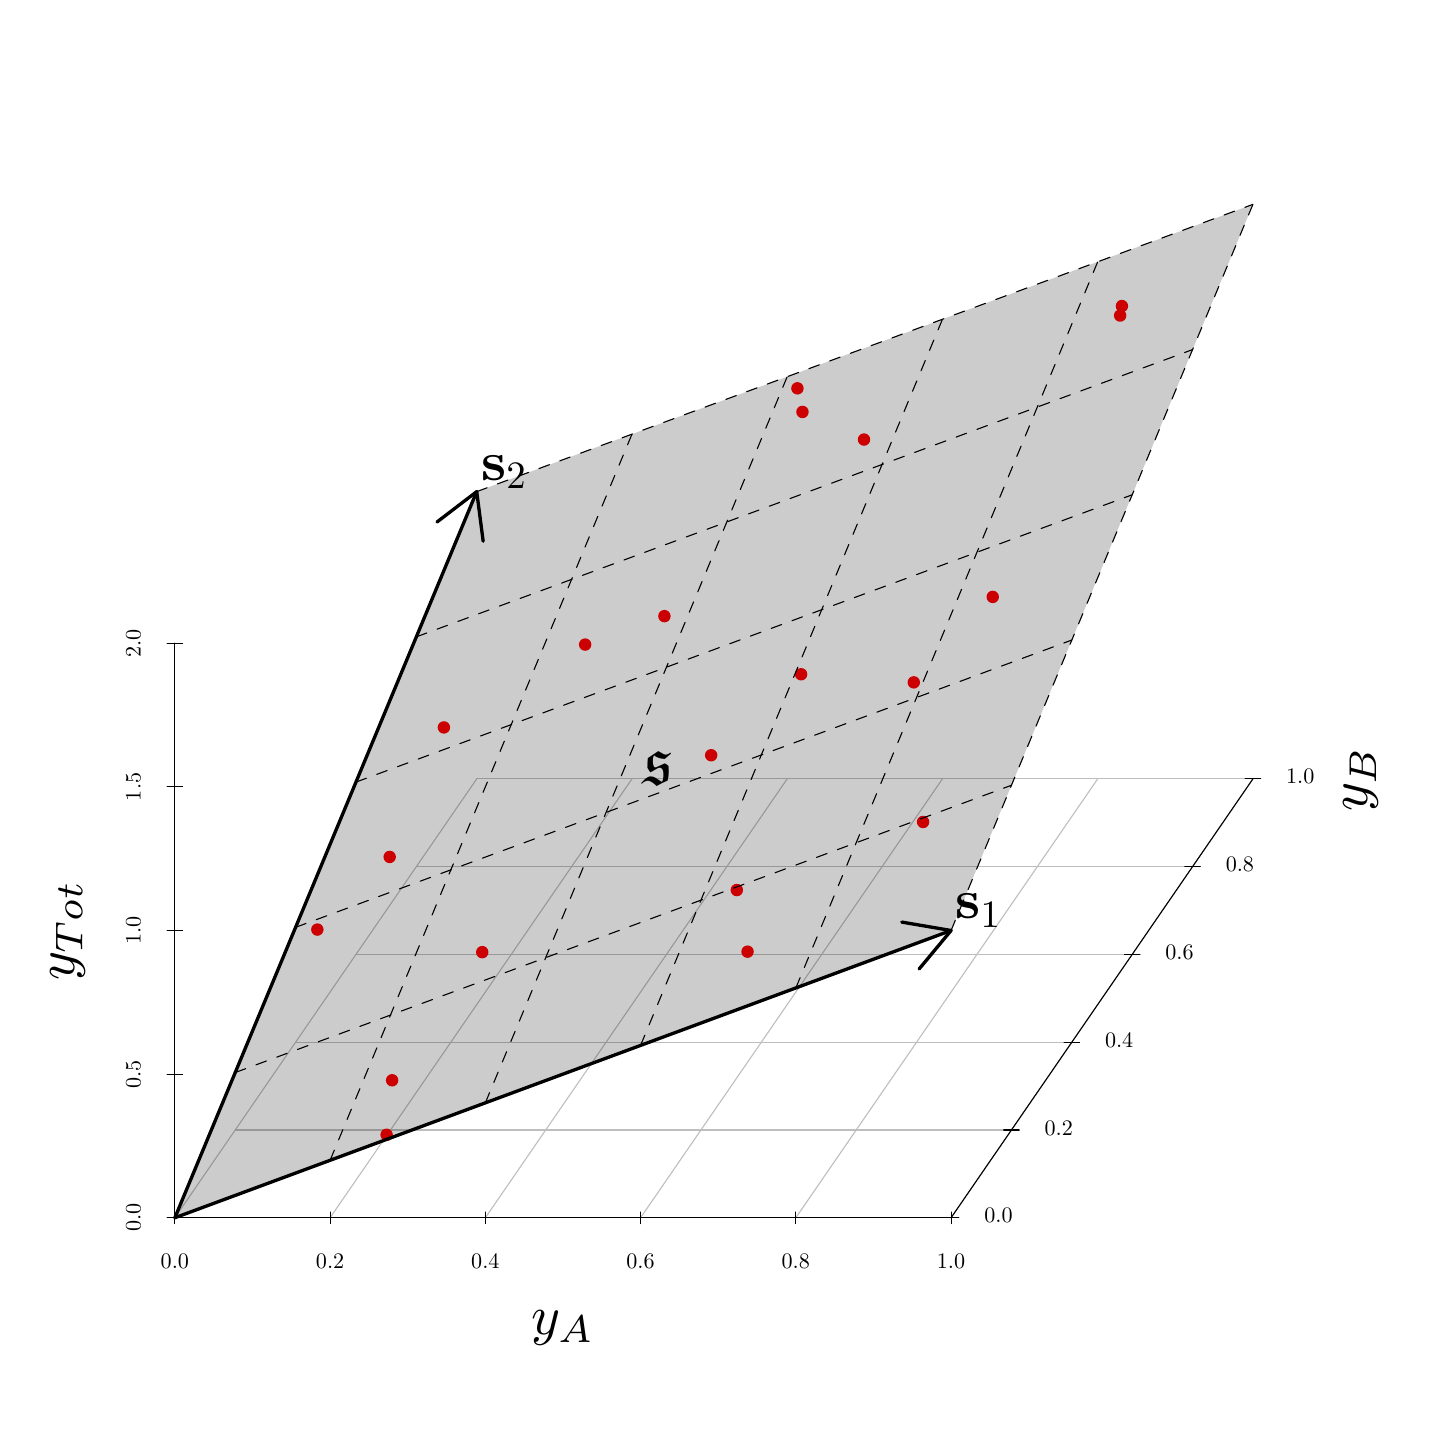
\begin{tikzpicture}[x=1pt,y=1pt]
\definecolor{fillColor}{RGB}{255,255,255}
\path[use as bounding box,fill=fillColor,fill opacity=0.00] (0,0) rectangle (505.89,505.89);
\begin{scope}
\path[clip] ( 37.20, 61.20) rectangle (468.69,456.69);
\definecolor{drawColor}{RGB}{190,190,190}

\path[draw=drawColor,line width= 0.4pt,line join=round,line cap=round] ( 53.18, 75.85) -- (162.26,234.44);

\path[draw=drawColor,line width= 0.4pt,line join=round,line cap=round] (109.28, 75.85) -- (218.36,234.44);

\path[draw=drawColor,line width= 0.4pt,line join=round,line cap=round] (165.38, 75.85) -- (274.45,234.44);

\path[draw=drawColor,line width= 0.4pt,line join=round,line cap=round] (221.47, 75.85) -- (330.55,234.44);

\path[draw=drawColor,line width= 0.4pt,line join=round,line cap=round] (277.57, 75.85) -- (386.65,234.44);

\path[draw=drawColor,line width= 0.4pt,line join=round,line cap=round] (333.67, 75.85) -- (442.74,234.44);

\path[draw=drawColor,line width= 0.4pt,line join=round,line cap=round] ( 53.18, 75.85) -- (333.67, 75.85);

\path[draw=drawColor,line width= 0.4pt,line join=round,line cap=round] ( 75.00,107.57) -- (355.48,107.57);

\path[draw=drawColor,line width= 0.4pt,line join=round,line cap=round] ( 96.81,139.28) -- (377.30,139.28);

\path[draw=drawColor,line width= 0.4pt,line join=round,line cap=round] (118.63,171.00) -- (399.11,171.00);

\path[draw=drawColor,line width= 0.4pt,line join=round,line cap=round] (140.44,202.72) -- (420.93,202.72);

\path[draw=drawColor,line width= 0.4pt,line join=round,line cap=round] (162.26,234.44) -- (442.74,234.44);
\definecolor{drawColor}{RGB}{0,0,0}

\path[draw=drawColor,line width= 0.4pt,line join=round,line cap=round] (330.86, 75.85) -- (336.47, 75.85);

\path[draw=drawColor,line width= 0.4pt,line join=round,line cap=round] (352.68,107.57) -- (358.29,107.57);

\path[draw=drawColor,line width= 0.4pt,line join=round,line cap=round] (374.49,139.28) -- (380.10,139.28);

\path[draw=drawColor,line width= 0.4pt,line join=round,line cap=round] (396.31,171.00) -- (401.92,171.00);

\path[draw=drawColor,line width= 0.4pt,line join=round,line cap=round] (418.12,202.72) -- (423.73,202.72);

\path[draw=drawColor,line width= 0.4pt,line join=round,line cap=round] (439.94,234.44) -- (445.55,234.44);

\path[draw=drawColor,line width= 0.4pt,line join=round,line cap=round] ( 53.18, 73.77) -- ( 53.18, 77.92);

\path[draw=drawColor,line width= 0.4pt,line join=round,line cap=round] (109.28, 73.77) -- (109.28, 77.92);

\path[draw=drawColor,line width= 0.4pt,line join=round,line cap=round] (165.38, 73.77) -- (165.38, 77.92);

\path[draw=drawColor,line width= 0.4pt,line join=round,line cap=round] (221.47, 73.77) -- (221.47, 77.92);

\path[draw=drawColor,line width= 0.4pt,line join=round,line cap=round] (277.57, 73.77) -- (277.57, 77.92);

\path[draw=drawColor,line width= 0.4pt,line join=round,line cap=round] (333.67, 73.77) -- (333.67, 77.92);

\path[draw=drawColor,line width= 0.4pt,line join=round,line cap=round] ( 50.38, 75.85) -- ( 55.99, 75.85);

\path[draw=drawColor,line width= 0.4pt,line join=round,line cap=round] ( 50.38,127.75) -- ( 55.99,127.75);

\path[draw=drawColor,line width= 0.4pt,line join=round,line cap=round] ( 50.38,179.65) -- ( 55.99,179.65);

\path[draw=drawColor,line width= 0.4pt,line join=round,line cap=round] ( 50.38,231.55) -- ( 55.99,231.55);

\path[draw=drawColor,line width= 0.4pt,line join=round,line cap=round] ( 50.38,283.45) -- ( 55.99,283.45);
\end{scope}
\begin{scope}
\path[clip] (  0.00,  0.00) rectangle (505.89,505.89);
\definecolor{drawColor}{RGB}{0,0,0}

\node[text=drawColor,anchor=base,inner sep=0pt, outer sep=0pt, scale=  0.80] at ( 53.18, 57.60) {0.0};

\node[text=drawColor,anchor=base,inner sep=0pt, outer sep=0pt, scale=  0.80] at (109.28, 57.60) {0.2};

\node[text=drawColor,anchor=base,inner sep=0pt, outer sep=0pt, scale=  0.80] at (165.38, 57.60) {0.4};

\node[text=drawColor,anchor=base,inner sep=0pt, outer sep=0pt, scale=  0.80] at (221.47, 57.60) {0.6};

\node[text=drawColor,anchor=base,inner sep=0pt, outer sep=0pt, scale=  0.80] at (277.57, 57.60) {0.8};

\node[text=drawColor,anchor=base,inner sep=0pt, outer sep=0pt, scale=  0.80] at (333.67, 57.60) {1.0};

\node[text=drawColor,rotate= 90.00,anchor=base,inner sep=0pt, outer sep=0pt, scale=  0.80] at ( 40.80, 75.85) {0.0};

\node[text=drawColor,rotate= 90.00,anchor=base,inner sep=0pt, outer sep=0pt, scale=  0.80] at ( 40.80,127.75) {0.5};

\node[text=drawColor,rotate= 90.00,anchor=base,inner sep=0pt, outer sep=0pt, scale=  0.80] at ( 40.80,179.65) {1.0};

\node[text=drawColor,rotate= 90.00,anchor=base,inner sep=0pt, outer sep=0pt, scale=  0.80] at ( 40.80,231.55) {1.5};

\node[text=drawColor,rotate= 90.00,anchor=base,inner sep=0pt, outer sep=0pt, scale=  0.80] at ( 40.80,283.45) {2.0};
\end{scope}
\begin{scope}
\path[clip] ( 37.20, 61.20) rectangle (468.69,456.69);
\definecolor{drawColor}{RGB}{0,0,0}

\node[text=drawColor,anchor=base west,inner sep=0pt, outer sep=0pt, scale=  0.80] at (345.67, 74.01) {0.0};

\node[text=drawColor,anchor=base west,inner sep=0pt, outer sep=0pt, scale=  0.80] at (367.48,105.73) {0.2};

\node[text=drawColor,anchor=base west,inner sep=0pt, outer sep=0pt, scale=  0.80] at (389.30,137.45) {0.4};

\node[text=drawColor,anchor=base west,inner sep=0pt, outer sep=0pt, scale=  0.80] at (411.11,169.16) {0.6};

\node[text=drawColor,anchor=base west,inner sep=0pt, outer sep=0pt, scale=  0.80] at (432.93,200.88) {0.8};

\node[text=drawColor,anchor=base west,inner sep=0pt, outer sep=0pt, scale=  0.80] at (454.74,232.60) {1.0};

\path[draw=drawColor,line width= 0.4pt,line join=round,line cap=round] ( 53.18, 75.85) --
	(333.67, 75.85);
\end{scope}
\begin{scope}
\path[clip] (  0.00,  0.00) rectangle (505.89,505.89);
\definecolor{drawColor}{RGB}{0,0,0}

\node[text=drawColor,anchor=base,inner sep=0pt, outer sep=0pt, scale=  2.00] at (193.42, 33.60) {$y_A$};
\end{scope}
\begin{scope}
\path[clip] ( 37.20, 61.20) rectangle (468.69,456.69);
\definecolor{drawColor}{RGB}{0,0,0}

\path[draw=drawColor,line width= 0.4pt,line join=round,line cap=round] (333.67, 75.85) --
	(442.74,234.44);
\end{scope}
\begin{scope}
\path[clip] (  0.00,  0.00) rectangle (505.89,505.89);
\definecolor{drawColor}{RGB}{0,0,0}

\node[text=drawColor,rotate= 90.00,anchor=base,inner sep=0pt, outer sep=0pt, scale=  2.00] at (484.29,234.44) {$y_B$};
\end{scope}
\begin{scope}
\path[clip] ( 37.20, 61.20) rectangle (468.69,456.69);
\definecolor{drawColor}{RGB}{0,0,0}

\path[draw=drawColor,line width= 0.4pt,line join=round,line cap=round] ( 53.18, 75.85) --
	( 53.18,283.45);
\end{scope}
\begin{scope}
\path[clip] (  0.00,  0.00) rectangle (505.89,505.89);
\definecolor{drawColor}{RGB}{0,0,0}

\node[text=drawColor,rotate= 90.00,anchor=base,inner sep=0pt, outer sep=0pt, scale=  2.00] at ( 16.80,179.65) {$y_{Tot}$};
\end{scope}
\begin{scope}
\path[clip] ( 37.20, 61.20) rectangle (468.69,456.69);
\definecolor{fillColor}{RGB}{255,0,0}

\path[fill=fillColor] (278.15,375.56) circle (  2.25);

\path[fill=fillColor] (279.97,367.03) circle (  2.25);

\path[fill=fillColor] (395.40,405.29) circle (  2.25);

\path[fill=fillColor] (394.76,401.87) circle (  2.25);

\path[fill=fillColor] (302.20,357.05) circle (  2.25);

\path[fill=fillColor] (201.44,282.97) circle (  2.25);

\path[fill=fillColor] (230.08,293.24) circle (  2.25);

\path[fill=fillColor] (150.40,253.03) circle (  2.25);

\path[fill=fillColor] (348.72,300.19) circle (  2.25);

\path[fill=fillColor] (279.47,272.24) circle (  2.25);

\path[fill=fillColor] (130.81,206.23) circle (  2.25);

\path[fill=fillColor] (246.98,242.98) circle (  2.25);

\path[fill=fillColor] (320.19,269.31) circle (  2.25);

\path[fill=fillColor] (104.67,179.99) circle (  2.25);

\path[fill=fillColor] (164.26,171.82) circle (  2.25);

\path[fill=fillColor] (256.24,194.27) circle (  2.25);

\path[fill=fillColor] (323.55,218.87) circle (  2.25);

\path[fill=fillColor] (131.69,125.53) circle (  2.25);

\path[fill=fillColor] (260.12,172.00) circle (  2.25);

\path[fill=fillColor] (129.70,105.84) circle (  2.25);
\definecolor{fillColor}{RGB}{0,0,0}

\path[fill=fillColor,fill opacity=0.20] ( 53.18, 75.85) --
	(162.26,338.24) --
	(442.74,442.04) --
	(333.67,179.65) --
	cycle;
\definecolor{drawColor}{RGB}{0,0,0}

\path[draw=drawColor,line width= 0.4pt,dash pattern=on 4pt off 4pt ,line join=round,line cap=round] ( 53.18, 75.85) -- (162.26,338.24);

\path[draw=drawColor,line width= 0.4pt,dash pattern=on 4pt off 4pt ,line join=round,line cap=round] (109.28, 96.61) -- (218.36,359.00);

\path[draw=drawColor,line width= 0.4pt,dash pattern=on 4pt off 4pt ,line join=round,line cap=round] (165.38,117.37) -- (274.45,379.76);

\path[draw=drawColor,line width= 0.4pt,dash pattern=on 4pt off 4pt ,line join=round,line cap=round] (221.47,138.13) -- (330.55,400.52);

\path[draw=drawColor,line width= 0.4pt,dash pattern=on 4pt off 4pt ,line join=round,line cap=round] (277.57,158.89) -- (386.65,421.28);

\path[draw=drawColor,line width= 0.4pt,dash pattern=on 4pt off 4pt ,line join=round,line cap=round] (333.67,179.65) -- (442.74,442.04);

\path[draw=drawColor,line width= 0.4pt,dash pattern=on 4pt off 4pt ,line join=round,line cap=round] ( 53.18, 75.85) -- (333.67,179.65);

\path[draw=drawColor,line width= 0.4pt,dash pattern=on 4pt off 4pt ,line join=round,line cap=round] ( 75.00,128.33) -- (355.48,232.13);

\path[draw=drawColor,line width= 0.4pt,dash pattern=on 4pt off 4pt ,line join=round,line cap=round] ( 96.81,180.80) -- (377.30,284.61);

\path[draw=drawColor,line width= 0.4pt,dash pattern=on 4pt off 4pt ,line join=round,line cap=round] (118.63,233.28) -- (399.11,337.09);

\path[draw=drawColor,line width= 0.4pt,dash pattern=on 4pt off 4pt ,line join=round,line cap=round] (140.44,285.76) -- (420.93,389.56);

\path[draw=drawColor,line width= 0.4pt,dash pattern=on 4pt off 4pt ,line join=round,line cap=round] (162.26,338.24) -- (442.74,442.04);

\path[draw=drawColor,line width= 1.2pt,line join=round,line cap=round] ( 53.18, 75.85) -- (333.67,179.65);

\path[draw=drawColor,line width= 1.2pt,line join=round,line cap=round] (322.13,165.75) --
	(333.67,179.65) --
	(315.86,182.69);

\path[draw=drawColor,line width= 1.2pt,line join=round,line cap=round] ( 53.18, 75.85) -- (162.26,338.24);

\path[draw=drawColor,line width= 1.2pt,line join=round,line cap=round] (164.59,320.32) --
	(162.26,338.24) --
	(147.91,327.26);

\node[text=drawColor,anchor=base west,inner sep=0pt, outer sep=0pt, scale=  2.00] at (335.27,183.85) {\bfseries s};

\node[text=drawColor,anchor=base west,inner sep=0pt, outer sep=0pt, scale=  1.40] at (344.34,180.84) {1};

\node[text=drawColor,anchor=base west,inner sep=0pt, outer sep=0pt, scale=  2.00] at (163.87,342.44) {\bfseries s};

\node[text=drawColor,anchor=base west,inner sep=0pt, outer sep=0pt, scale=  1.40] at (172.94,339.43) {2};

\node[text=drawColor,anchor=base west,inner sep=0pt, outer sep=0pt, scale=  1.00] at (222.57,232.24) {{\Huge $\mathfrak{s}$}};
\end{scope}
\end{tikzpicture}

   }
   \caption{Depiction of a three dimensional hierarchy with $y_{\text{Tot}} = y_{\text{A}} + y_{\text{B}}$. The gray coloured two dimensional plane depicts the coherent subspace $\mathfrak{s}$ where $\vec{s}_1 = (1,1,0)'$ and $\vec{s}_2 = (1, 0, 1)'$ are basis vectors that span $\mathfrak{s}$. The red points in $\mathfrak{s}$ represent realisations or coherent forecasts.}\label{fig:3D_hierarchy}
\end{figure}

\begin{definition}[Hierarchical Time Series]\label{def:hts}
   A hierarchical time series is an $n$-dimensional multivariate time series such that all observed values $\bm{y}_1,\ldots,\bm{y}_T$ and all future values $\bm{y}_{T+1},\bm{y}_{T+2},\ldots$ lie in the coherent subspace, i.e., $\bm{y}_t\in\mathfrak{s}\quad\forall t$.
\end{definition}

Despite the common use of the term \emph{hierarchical time series}, it should be clear from the definition that the data need not necessarily follow a hierarchy. Also notable by its absence in the above definition is any reference to \emph{aggregation}. In some ways, terms such as \emph{hierarchical} and \emph{aggregation} can be misleading since the literature has covered instances that cannot be depicted in a similar fashion to Figure~\ref{fig:basichier} and/or do not involve aggregation. Examples include, temporal hierarchies which involve grouped structures \citep[see][]{AthEtAl2017}, overlapping temporal hierarchies \citep[see][]{JeoEtAl2019}, applications for which the difference rather than the aggregate is of interest \cite[see][]{LiTan2019}, or structures that involve both cross-sectional and temporal dimensions referred to as cross-temporal structures \citep[see][]{KouAth2019}. Finally, although Definition~\ref{def:hts} makes reference to time series, this definition can be easily generalised to any vector-valued data for which some linear constraints are known to hold for all realisations.

%  It will sometimes be useful to think of pre-multiplication by $\bm{S}$ as a mapping from $\mathbb{R}^m$ to $\mathbb{R}^n$, in which case we use the notation $s(.)$. Although the codomain of $s(.)$ is $\mathbb{R}^n$, its image is the coherent space $\mathfrak{s}$ as depicted in Figure~\ref{fig2}.
%
%  \begin{figure}[H]
%    \begin{center}
%      \begin{tikzpicture}[
%      >=stealth,
%      bullet/.style={
%        fill=black,
%        circle,
%        minimum width=1.5cm,
%        inner sep=0pt
%      },
%      projection/.style={
%        ->,
%        thick,
%        label,
%        shorten <=2pt,
%        shorten >=2pt
%      },
%      every fit/.style={
%        ellipse,
%        draw,
%        inner sep=0pt
%      }
%      ]
%      \node at (2,3) {$s$};
%      \node at (0,5) {$\mathbb{R}^m$(domain of $s$)};
%      \node at (4,5) {$\mathbb{R}^n$(codomain of $s$)};
%      \node at (4.7,2.0) {$\mathfrak{s}$(image of $s$)};
%      %\node[bullet,label=below:$f(x)$] at (4,2.5){};
%      \draw (0,2.5) ellipse (1.02cm and 2.2cm);
%      \draw (4,2.5) ellipse (1.02cm and 2.2cm);
%      \draw (4,2.5) ellipse (0.51cm and 1.1cm);
%      \draw[projection, label=below:$f$] (0.3,2.5) -- (3.8,2.5) ;
%      \end{tikzpicture}
%    \end{center}
%    \caption{The domain, codomain and image of the mapping $s$.}\label{fig2}
%  \end{figure}

\begin{definition}[Coherent Point Forecasts]\label{def:cohpoint}
  Let $\breve{\bm{y}}_{t+h|t} \in \mathbb{R}^n$ be a vector of point forecasts of all series in the hierarchy where the subscript $t+h|h$ implies that the forecast is made as time $t$ for a period $h$ steps into the future. Then $\breve{\bm{y}}_{t+h|t}$ is \emph{coherent} if $\breve{\bm{y}}_{t+h|t} \in \mathfrak{s}$.
\end{definition}

Without any loss of generality, the above definition could also be applied to prediction for multivariate data in general, rather than just forecasting of time series.

Much of the early literature that dealt with the problem of forecasting hierarchical time series \citep[see][and references therein]{Gross1990} produced forecasts at a single level of the hierarchy in the first stage. Subsequently forecasts for all series were recovered through {\color{blue} either} aggregation, disaggregation according to historical or forecast proportions, or some combination of both. Consequently, incoherent forecasts were not a problem in these earlier papers.

Forecasting a single level of the hierarchy did not echo common practice within many industries. In many organisations different departments or `silos' each produced their own forecasts, often with their own information sets and judgemental adjustments.\footnote{\citet{Cha2013} discusses silos and the importance of information and data sharing across an organisation.} This approach does have several advantages over only forecasting a single level. First, there is no loss of information since all levels and series are modelled. Second, modelling higher level series often identifies features such as trend and seasonality that cannot be detected in noisy disaggregate data. However, when forecasts are produced independently at all levels, forecasts are likely to be incoherent.\footnote{There are some special cases of using simple approaches such as na\"{i}ve, which extrapolate the coherent nature of the data to the forecasts.} {\color{blue}While the problem of incoherent forecasts can be addressed by some multivariate approaches, including state space models, these can not always be generalised to models with more complicated features or scaled up to high-dimensional problems.}  Instead, the solution is to make an adjustment, {\color{blue}ex post of base forecasting,} that ensures coherence, a process known as \emph{forecast reconciliation}

\section{Forecast reconciliation}\label{sec:Reconciliation}

The concept of forecast reconciliation is predicated on there being an $n$-vector of forecasts that are incoherent. We call these \emph{base forecasts} and denote them as $\hat{\bm{y}}_{t+h|t}$. In the sequel, this subscript will be dropped at times for ease of exposition. In the most general terms, reconciliation can be defined as follows.

\begin{definition}[Reconciled forecasts]\label{def:reconpoint}
  Let $\psi$ be a mapping, $\psi:\mathbb{R}^n\rightarrow\mathfrak{s}$. The point forecast $\tilde{\bm{y}}_{t+h|t}=\psi(\hat{\bm{y}}_{t+h|t})$ ``reconciles'' a base forecast $\hat{\bm{y}}_{t+h|t}$ with respect to the mapping $\psi(.)$
\end{definition}

All reconciliation methods that we are aware of consider a linear mapping for $\psi$, which involves pre-multiplying base forecasts by an $n\times n$ matrix that has $\mathfrak{s}$ as its image. One way to achieve this is with a matrix $\bm{S}\bm{G}$, where $\bm{G}$ is an $m\times n$ matrix (some authors use $\bm{P}$ in place of $\bm{G}$). This facilitates an interpretation of reconciliation as a two-step process. In the first step, base forecasts $\hat{\bm{y}}_{t+h|t}$ are combined to form a new set of bottom-level forecasts. In the second step, these are mapped to a full vector of coherent forecasts via pre-multiplication by $\bm{S}$.

Although pre-multiplying base forecasts by $\bm{S}\bm{G}$ will result in coherent forecasts, a number of desirable properties arise when $\bm{S}\bm{G}$ has the specific structure of a \emph{projection} matrix onto $\mathfrak{s}$. In general a projection matrix is defined via its idempotence property, i.e. $(\bm{S}\bm{G})^2=\bm{S}\bm{G}$. We also rely on another property of projection matrices, namely that any vector lying in the image of a projection is mapped to itself by that projection \citep[see Lemma 2.4 in][for a proof]{rao1974}. In our context this implies that for any $\bm{v}\in\mathfrak{s}$, $\bm{S}\bm{G}\bm{v}=\bm{v}$.

We begin by considering the special case of an orthogonal projection whereby $\bm{G}=(\bm{S}'\bm{S})^{-1}\bm{S}'$. This is equivalent to so called OLS reconciliation as introduced by \citet{Hyndman2011}. We refrain from any discussion of regression models focusing instead on geometric interpretations. {\color{blue} Nonetheless,} the connection between OLS and orthogonal projection should be clear in the context of regression modelling predicted values from OLS are obtained via an orthogonal projection of the response onto the span of the regressors.


\subsection{Orthogonal projection}\label{sec:orthogonal}

In this section we discuss two sensible properties that can be achieved by reconciliation via orthogonal projection.
\begin{enumerate}
\item The first is that reconciliation should adjust the base forecasts as little as possible; i.e. the base and reconciled forecasts should be `close'.
\item The second is that reconciliation in some sense should improve forecast accuracy, or more loosely, that the reconciled forecast should be `closer' to the realised value targeted by the forecast.
\end{enumerate}

To address the first of these properties we make the concept of closeness more concrete by considering the Euclidean distance between the base forecast $\hat{\bm{y}}_{t+h|t}$ and the reconciled forecast $\tilde{\bm{y}}_{t+h|t}$. A property of an orthogonal projection is that the distance between $\hat{\bm{y}}_{t+h|t}$ and $\tilde{\bm{y}}_{t+h|t}$ is minimal over any possible $\tilde{\bm{y}}_{t+h|t}\in\mathfrak{s}$. In this sense reconciliation via orthogonal projection {\color{blue} $\bm{G}=(\bm{S}'\bm{S})^{-1}\bm{S}'$} leads to the smallest possible adjustments of the base forecasts.  {\color{blue} ALternatively, Euclidean distance can be interpreted as a loss function $L(\bm{u},\bm{v})=\|\bm{u}-\bm{v}\|$ where $\|.\|$ denotes the L2 norm, in which case an orthogonal projection solves the optimisation problem $\underset{\bm{G}}{\min}\,L(\bm{S}\bm{G}\hat{\bm{y}}_{t+h|t},\hat{\bm{y}}_{t+h|t})$. This is a special case of the optimisation problem considered by \cite{NysEtAl2019}, the more general case will be covered in the next section.}

The {\color{blue} aim of the second property is to guarantee that} reconciled forecasts should always be closer to the target than base forecasts {\color{blue} and is related to the difference in loss functions $L({\bm{y}}_{t+h},\hat{\bm{y}}_{t+h|t})-L({\bm{y}}_{t+h},\tilde{\bm{y}}_{t+h|t})$.  This is expressed as a minimax optimisation by \cite{VanErven2015a} and was also} touched upon in Section 2.3 of \citet{WicEtAl2019}{\color{blue}, albeit in both cases for a slightly different loss function}. Here we provide a new explicit proof of {\color{blue} this distance reducing property}. We do so first in the case {\color{blue} of the loss function defined here in terms of Euclidean distance} where the geometric intuition of the proof is clear and then generalise the result to {\color{blue} more general loss functions} Section~\ref{sec:oblique}

Consider the Euclidean distance between the target and a forecast. This is equivalent to the square root of the sum of squared forecast errors over the entire hierarchy. Let $\bm{y}_{t+h}$ be the realisation of the data generating process at time $t+h$. The following theorem shows that reconciliation never increases the sum of squared errors of point forecasts.

\begin{theo}[Distance reducing property]\label{th:distred}
  If $\tilde{\bm{y}}_{t+h|t}=\bm{S}\bm{G}\hat{\bm{y}}_{t+h|t}$, where $\bm{G}$ is such that $\bm{S}\bm{G}$ is an orthogonal projection (in the Euclidean sense) onto $\mathfrak{s}$ then:
  \begin{equation*}
    \|(\bm{y}_{t+h}-\tilde{\bm{y}}_{t+h|t})\|\le\|(\bm{y}_{t+h}-\hat{\bm{y}}_{t+h|t})\|.
  \end{equation*}
\end{theo}
\begin{proof}
  Since $\bm{y}_{t+h|t},\tilde{\bm{y}}_{t+h|t}\in\mathfrak{s}$ and since the projection is orthogonal, by Pythagoras' theorem
  \begin{equation*} \|(\bm{y}_{t+h}-\hat{\bm{y}}_{t+h|t})\|^2=\|(\bm{y}_{t+h}-\tilde{\bm{y}}_{t+h|t})\|^2+\|(\tilde{\bm{y}}_{t+h|t}-\hat{\bm{y}}_{t+h|t})\|^2.
  \end{equation*}

  Since $\|(\tilde{\bm{y}}_{t+h|t}-\hat{\bm{y}}_{t+h|t})\|^2\ge 0$ this implies,
  \begin{equation*} \|(\bm{y}_{t+h}-\hat{\bm{y}}_{t+h|t})\|^2\ge\|(\bm{y}_{t+h}-\tilde{\bm{y}}_{t+h|t})\|^2,
  \end{equation*}
  with equality only holding when $\tilde{\bm{y}}_{t+h|t}=\hat{\bm{y}}_{t+h|t}$. Taking the square root of both sides proves the desired result.
\end{proof}

The simple geometric intuition behind the proof is demonstrated in Figure~\ref{fig:Schematic_OLSRecon}. In this schematic, the coherent subspace is depicted as a black arrow, and the base forecast $\hat{\bm{y}}$ is shown as a blue dot. Since $\hat{\bm{y}}$ is incoherent, $\hat{\bm{y}}\notin\mathfrak{s}$ and in this case the inequality is strict. Reconciliation is an orthogonal projection from $\hat{\bm{y}}$ to the coherent subspace yielding the reconciled forecast $\tilde{\bm{y}}$ shown in red. Finally, the target of the forecast $\bm{y}$ is displayed as a black point, and although its exact location is unknown to the forecaster, it is known that it will lie somewhere along the coherent subspace.

\begin{figure}[!hbt]
  \centering 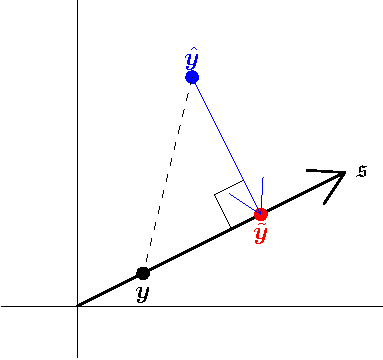
\includegraphics[width=0.6\textwidth]{Figs/orth_pointforerec_schematic.pdf}
  \caption{Orthogonal projection of $\hat{\bm{y}}$ onto $\mathfrak{s}$ yielding the reconciled forecast $\tilde{\bm{y}}$.}\label{fig:Schematic_OLSRecon}
\end{figure}

Figure~\ref{fig:Schematic_OLSRecon} clearly shows that $\hat{\bm{y}}$, $\tilde{\bm{y}}$ and $\bm{y}$ form a right angled triangle with $\tilde{\bm{y}}$ at the right-angled vertex. In this triangle, the line between $\bm{y}$ and $\hat{\bm{y}}$ is the hypotenuse and therefore must be longer than the distance between $\bm{y}$ and $\tilde{\bm{y}}$. Therefore reconciliation is guaranteed to reduce {\color{blue} a loss function based on distance, or indeed any monotonic function of distance.}

Theorem~\ref{th:distred} is in some ways more powerful than perhaps previously understood. Crucially, the result is not a result that requires taking expectations. This distance reducing property will hold for any realisation and any forecast and not just on average. Nothing needs to be assumed about the statistical properties of the data generating process or the process by which forecasts are made.

In other ways, Theorem~\ref{th:distred} is weaker than perhaps often understood. First, when improvements in forecast accuracy are discussed in the context of the theorem, this refers to a very specific measure of forecast accuracy. In particular, this measure is the sum of squared forecast errors of \emph{all} variables in the hierarchy {\color{blue}(or any monotonic function thereof)}.  Second, although an orthogonal projection is guaranteed to improve on base forecasts, it is not necessarily the projection that leads to the greatest improvement in forecast accuracy in expectation. Therefore, referring to OLS reconciliation as `optimal' is somewhat misleading since it does not have the optimality properties of some oblique projections. {\color{blue} We now turn our attention to the way oblique projections can address both of these shortcomings.}

\subsection{Oblique Projections}\label{sec:oblique}

One justification for using an orthogonal projection is that it leads to improved forecast accuracy in terms of {\color{blue} a loss function based on Euclidean distance that involves \emph{all} variables in the hierarchy.} A clear shortcoming of this measure of forecast accuracy is that forecast errors in all series should not necessarily be treated equally. For example, in hierarchies, top-level series tend to have a much larger scale than bottom-level series.  {\color{blue} Alternatively, the context of the forecast problem itself may suggest a loss function that weights series differently.  For example in our tourism application in Section~\ref{sec:EmpStudy} we will consider weighting forecast errors by average tourism expenditure in each region.}\footnote{Similar consideration are taken into account for the loss function used in the M5 forecasting competition, see M5 REF HERE for more details. Add Athanasopoulos and Kourentzes (2020) discussion paper}  An even more sophisticated understanding may take {\color{blue}linear combinations} of series into account. All of these considerations lead towards {\color{blue} a loss function $L_{\bm W}(\bm{y}_{t+h},\tilde{\bm{y}}_{t+h|t})=||{\bm{y}_{t+h}-\tilde{\bm{y}}_{t+h|t}}||_{\bm{W}}$ where $||\bm{v}||_{\bm{W}}=\bm{v}'\bm{W}\bm{v}$, and $\bm{W}$ is a symmetric matrix assumed to be invertible.  The geometry defined by the norm $||.||_{\bm{W}}$, will be referred to as the generalised Euclidean geometry with respect to $\bm{W}$. }

One way to understand the generalised Euclidean geometry is that it is the same as Euclidean geometry when all vectors are first transformed by pre-multiplying by $\bm{W}^{1/2}$, {\color{blue} where $\bm{W}=(\bm{W}^{1/2})'\bm{W}^{1/2}$}. This leads to a transformed $\bm{S}$ matrix $\bm{S}^*=\bm{W}^{1/2}\bm{S}$ and transformed $\hat{\bm{y}}$ and $\tilde{\bm{y}}$ vectors $\hat{\bm{y}}^*=\bm{W}^{1/2}\hat{\bm{y}}$ and $\tilde{\bm{y}}^*=\bm{W}^{1/2}\tilde{\bm{y}}$. {\color{blue} A projection of the form $\tilde{\bm{y}}=\bm{S}(\bm{S}'\bm{W}\bm{S})^{-1}\bm{S}'\bm{W}\hat{\bm{y}}$, is an} orthogonal projection in the transformed space since
\begin{align*}
  \tilde{\bm{y}}^*
    & = \bm{W}^{1/2}\tilde{\bm{y}} \\
    & = \bm{W}^{1/2}\bm{S}(\bm{S}'\bm{W}\bm{S})^{-1}\bm{S}'\bm{W}\hat{\bm{y}} \\
    &{\color{blue} = \bm{W}^{1/2}\bm{S}((\bm{W}^{1/2}\bm{S})'\bm{W}^{1/2}\bm{S})^{-1}(\bm{W}^{1/2}\bm{S})'\bm{W}^{1/2}\hat{\bm{y}}}\\
    & = \bm{S}^*(\bm{S}^{*'}\bm{S}^*)^{-1}\bm{S}^{*'}\hat{\bm{y}^*}.
\end{align*}

%Thinking of the problem in terms of a geometry defined by the norm $\bm{v}'\bm{W}^{-1}\bm{v}$ is also quite instructive when it comes to thinking about the connection between distances and loss functions. In the generalised Euclidean geometry, the distance between the reconciled forecast and the realisation is given by $(\bm{y}-\hat{\bm{y}})'\bm{W}^{-1}(\bm{y}-\hat{\bm{y}})$. For diagonal $\bm{W}^{-1}$, this is equivalent to a weighted sum of squared error loss function and when $\bm{W}$ is a covariance matrix, this is equivalent to a Mahalanobis distance. Therefore Theorem~\ref{th:distred} can easily be generalised as follows.

Thinking of the generalised Euclidean space as a transformed version of Euclidean space also allows the distance reducing property of Theorem~\ref{th:distred} to be generalised to any loss function $L_{\bm{W}}$

\begin{theo}[General distance reducing property]\label{th:gdistred}
  If $\tilde{\bm{y}}_{t+h|t}=\bm{S}\bm{G}\hat{\bm{y}}_{t+h|t}$, where $\bm{G}$ is such that $\bm{S}\bm{G}$ is an orthogonal projection (in the generalised Euclidean sense) onto $\mathfrak{s}$ then:
  \begin{equation*}
    \|(\bm{y}_{t+h}-\tilde{\bm{y}}_{t+h|t})\|_{\bm{W}}
      \le\
    \|(\bm{y}_{t+h}-\hat{\bm{y}}_{t+h|t})\|_{\bm{W}}.
  \end{equation*}
\end{theo}
\begin{proof}
  The proof is identical to the proof for Theorem~\ref{th:distred} but relies on the Generalised Pythagorean Theorem (applicable to Generalised Euclidean space) rather than the Pythagorean Theorem.
  \end{proof}

The implication of Theorem~\ref{th:gdistred} is that if the loss function is a monotonic function of $L_{\bm{W}}$ {\color{blue} with some $\bm{W}$ given a priori} then the projection matrix $\bm{S}(\bm{S}'\bm{W}^{-1}\bm{S})^{-1}\bm{S}'\bm{W}^{-1}$ is guaranteed to improve forecast accuracy over base forecasts.  {\color{blue}  This result does not necessarily involve the covariance of forecast errors unless $\bm{W}$ is explicitly chosen to depend on these covariances.}

\citet{WicEtAl2019} and \citet{VanErven2015a} both prove special cases of this result, the former in the case where $\bm{W}$ is the inverse of the forecast error covariance and the latter in the case where $\bm{W}$ is diagonal.  Note here that we rely here on the Generalised Pythagorean Theorem (which involves an equality). In contrast, \citet{WicEtAl2019} follow \citet{VanErven2015a} in stating their result in terms of the Generalised Pythagorean Inequality. These proofs require an assumption of convexity so that the angle between the base forecast and coherent subspace must be greater than 90 degrees. The proof we have provided here requires no such assumption, since this may not hold for an arbitrary $\bm{W}$. As such the statement from \citet{WicEtAl2019} that \emph{``MinT reconciled forecasts are at least as good as the incoherent forecasts''} should be qualified --- this is true only for loss {\color{blue}that is a monotonic function of $L_{\bm{\Sigma}^{-1}}$, where $\bm{\Sigma}=E(\bm{y}-\hat{\bm{y}})(\bm{y}-\hat{\bm{y}})'$}. If Euclidean distance (or mean squared error) is used {\color{blue} as a loss function}, there will be realisations where the MinT estimator does not improve forecast accuracy relative to base forecasts. This will be demonstrated using a real data set in the empirical study in Section~\ref{sec:comparebase}.

\subsection{MinT}

{\color{blue}The discussion so far provides a roadmap, such that for a given choice of $\bm{W}$, a projection with distance-reducing properties can be derived}. While the MinT method of \citet{WicEtAl2019} {\color{blue} is a special case of such a projection, it was in fact motivated by a different optimality property.  This was to minimise the} trace of the forecast error covariance matrix of reconciled forecasts, i.e,
	
{\color{blue}
\begin{equation}
\label{eq:MinTObj}
\underset{\bm{G}}{\min}\,\textrm{tr}(E\left[(\bm{y}-{\bm S}{\bm G}\hat{\bm{y}})(\bm{y}-{\bm S}{\bm G}\hat{\bm{y}})'\right])\,.
\end{equation}
}

The solution is the oblique projection {\color{blue} $\bm{S}\left(\bm{S}'\bm{\Sigma}^{-1}\bm{S}\right)^{-1}\bm{S}'\bm{\Sigma}^{-1}$}. {\color{blue} While MinT is used here to refer to the case where $\bm{\Sigma}$ is known, in practice,} it is unknown.  It can be estimated using in-sample errors, {\color{blue} with some specific estimators found in \cite{WicEtAl2019} and also \cite{NysEtAl2019}.}

Figure~\ref{fig:OthogonalVSOblique_projection} provides geometrical intuition into the MinT method. Suppose that the orange points in panel~(a) represent in-sample forecast errors. These provide information on the most likely direction of large deviations from the coherent subspace $\mathfrak{s}$. This direction is denoted by $\bm{R}$. Panel~(b) shows a target value of $\bm{y}$, while the grey points indicate possible values for the base forecasts (the base forecasts are of course stochastic). One possible value of the forecast is depicted in blue as $\hat{\bm{y}}$. An oblique projection of the blue point back along the direction of $\bm{R}$, yields a reconciled forecast closer to the target, especially compared to an orthogonal projection. Panel~(c) shows the orthogonal projection of every potential base forecast onto the coherent subspace. Panel~(d) depicts an oblique projection along $\bm{R}$ for all the gray points. The oblique projection yields reconciled forecasts tightly packed near the target $\bm{y}$. In this sense, the oblique MinT projection minimises the forecast error variance of the reconciled forecasts. In contrast to the result in Theorem~\ref{th:gdistred}, this property is a statistical property in the sense that MinT is optimal in expectation.

\begin{figure}[!p]
  \centering
  \begin{subfigure}[!h]{0.415\textwidth}
      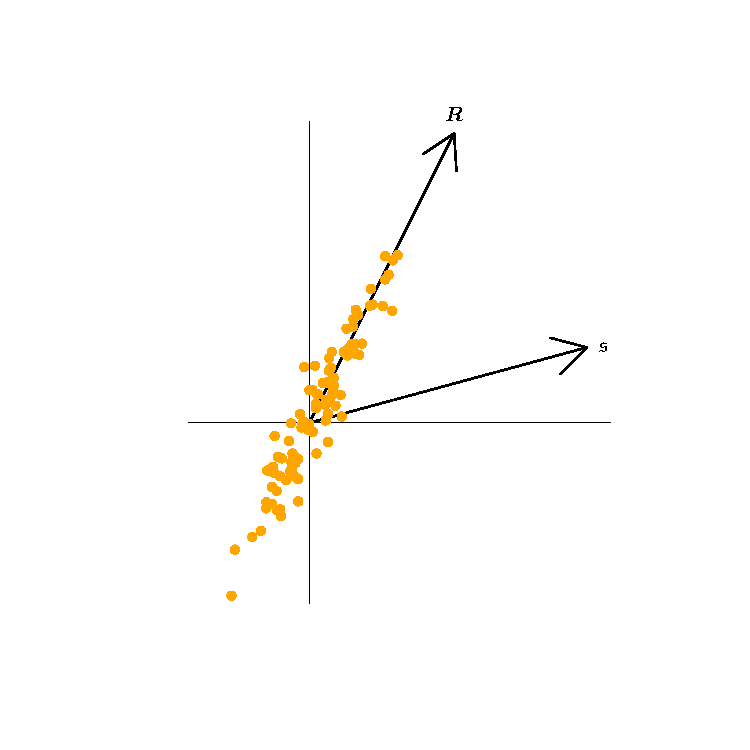
\includegraphics[width=\textwidth]{Figs/InsampDir_1_George.pdf}
      \caption{}
  \end{subfigure}
  \begin{subfigure}[!h]{0.415\textwidth}
      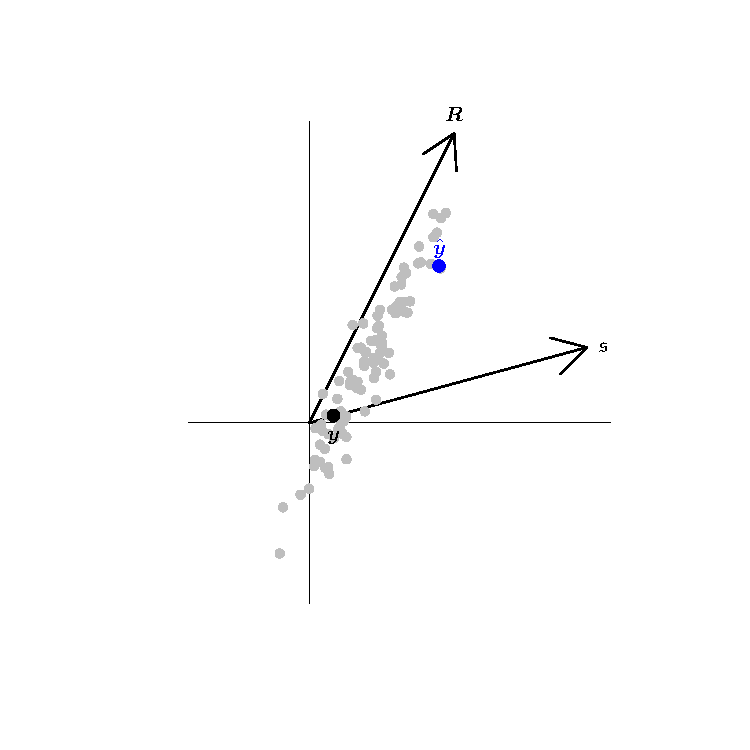
\includegraphics[width=\textwidth]{Figs/InsampDir_2_George.pdf}
      \caption{}
  \end{subfigure}
  \begin{subfigure}[!h]{0.415\textwidth}
      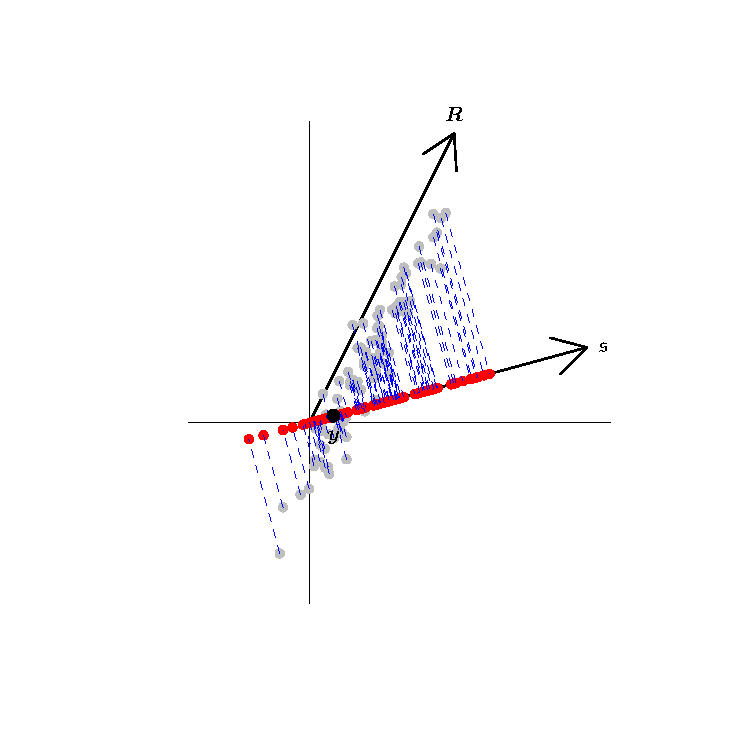
\includegraphics[width=\textwidth]{Figs/OrthProj_George.pdf}
      \caption{}
  \end{subfigure}
  \begin{subfigure}[!h]{0.415\textwidth}
      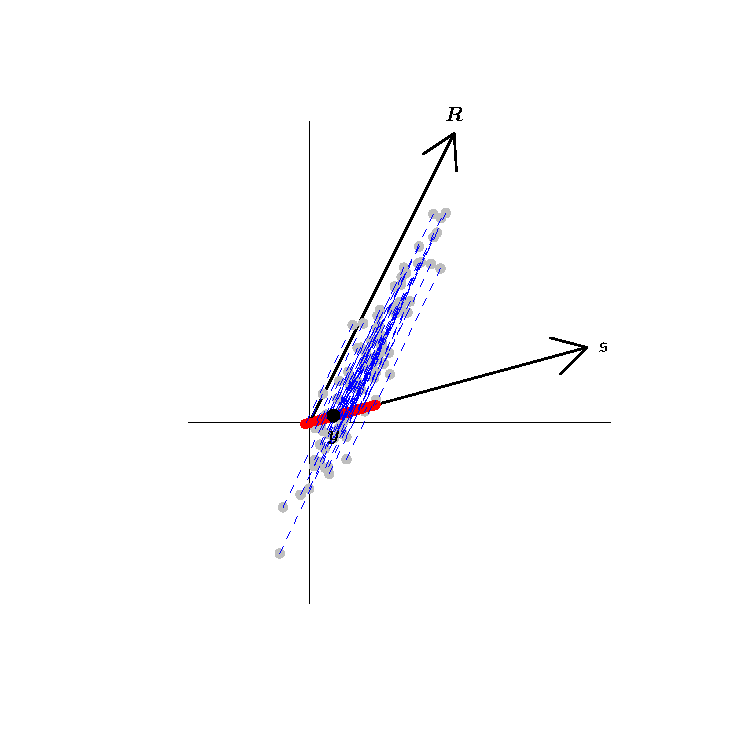
\includegraphics[width=\textwidth]{Figs/ObliqProj_George.pdf}
      \caption{}
  \end{subfigure}
  \caption{A schematic represention of orthogonal and oblique reconciliations. The orange points in (a) represent in-sample errors and $\bm{R}$ shows the most likely direction of deviations from the coherent subspace $\mathfrak{s}$. Grey points in (b) indicate potential base forecasts while the blue dot ${\hat{\bm y}}$ represents one such realisation. The black dot ${\bm y}$ denotes the (unknown) target of the forecast. (c) shows the orthogonal projection of all potential base forecasts onto the coherent subspace while (d) shows an oblique projection.}\label{fig:OthogonalVSOblique_projection}
\end{figure}

{\color{blue}

\subsection{Expected loss minimisation and MinT}

We now make explicit the connection between MinT and a loss function based on the squared Euclidean distance $L^2(\bm{y},\tilde{\bm{y}})=\|\bm{y}-\tilde{\bm{y}}\|^2$ before generalising to $L^2_{\bm W}(\bm{y},\tilde{\bm{y}})=\|\bm{y}-\tilde{\bm{y}}\|^2_{\bm W}$.  \footnote{Since taking the square is monotonic over the range of $L$ and $L_{\bm W}$, the properties in Theorem~\ref{th:distred} and Theorem~\ref{th:gdistred} also apply to $L^2$ and $L^2_{\bm W}$.}  By the properties of the trace operator, the objective function in Eq.~\eqref{eq:MinTObj} can be rearranged as

\begin{align*}
\label{eq:MinTObj}
\textrm{tr}(E\left[(\bm{y}-{\bm S}{\bm G}\hat{\bm{y}})(\bm{y}-{\bm S}{\bm G}\hat{\bm{y}})'\right])&=\textrm{tr}(E\left[(\bm{y}-{\bm S}{\bm G}\hat{\bm{y}})'(\bm{y}-{\bm S}{\bm G}\hat{\bm{y}})\right])\\
%&=E\left[(\bm{y}-{\bm S}{\bm G}\hat{\bm{y}})'(\bm{y}-{\bm S}{\bm G}\hat{\bm{y}})\right]\\
&=E\left[\|\bm{y}-{\bm S}{\bm G}\hat{\bm{y}}\|^2\right]\\
&=E\left[L^2(\bm{y},\tilde{\bm{y}})\right]
\end{align*}

Note that trace minimisation implies a different optimality property to the distance reducing property described in Section~\ref{sec:orthogonal}.  Theorem~\ref{th:distred} implies optimality in the sense that reconcilied forecasts always improve on base forecasts.  For MinT, optimality refers to minimising the loss function \textit{in expectation}.

Suppose the optimisation problem is generalised to a loss function based on some ${\bm W}$

{\color{blue}
	\begin{equation}
	\label{eq:GMinTObj}
	\underset{\bm{G}}{\min}\,(E\left[(\bm{y}-{\bm S}{\bm G}\hat{\bm{y}})'\bm{W}(\bm{y}-{\bm S}{\bm G}\hat{\bm{y}})\right])\,.
	\end{equation}
}

The following theorem proves that the solution to this optimisation problem does not depend of the choice of $\bm{W}$ used in the loss function.

\begin{theo}[Expected loss minimisation and MinT]\label{th:gmint}
    The usual MinT reconciliation method $\tilde{\bm{y}}=\bm{S}\left(\bm{S}'\bm{\Sigma}^{-1}\bm{S}\right)^{-1}\bm{S}'\bm{\Sigma}^{-1}\hat{\bm{y}}$ solves the optimisation problem in Eq.~\eqref{eq:GMinTObj} for any choice of $\bm{W}$.
\end{theo}
\begin{proof}
	The loss function in Eq.~\eqref{eq:GMinTObj} is equivalent to Euclidean distance in the transformed space and can therefore be minimised by using the MinT method in this space. The MinT method in the transformed space is given by
	\begin{equation}
	\label{eq:MinTtran}
	\tilde{\bm{y}}^{*}=\bm{S}^{*}\left(\bm{S}^{*'}\bm{\Sigma}^{*-1}\bm{S}^{*}\right)^{-1}\bm{S}^{*'}\bm{\Sigma}^{*-1}\hat{\bm{y}}^{*}\,,
	\end{equation}
	where  $\bm{y}^{*}=\bm{W}^{1/2}\bm{y}$, $\bm{S}^{*}=\bm{W}^{1/2}\bm{S}$, $\hat{\bm{y}}^{*}=\bm{W}^{1/2}\hat{\bm{y}}$ and
	\begin{align*}
	\bm{\Sigma}^*&=E\left[(\bm{y}^{*}-\hat{\bm{y}}^{*})(\bm{y}^{*}-\hat{\bm{y}}^{*})'\right]\\
	&=E\left[\bm{W}^{1/2}(\bm{y}-\hat{\bm{y}})(\bm{y}-\hat{\bm{y}})'(\bm{W}^{1/2})'\right]\\
	&=\bm{W}^{1/2}E\left[(\bm{y}-\hat{\bm{y}})(\bm{y}-\hat{\bm{y}})'\right](\bm{W}^{1/2})'\\
	&=\bm{W}^{1/2}\bm{\Sigma}(\bm{W}^{1/2})'
	\end{align*}
	Noting that
	\begin{align*}
	(\bm{\Sigma}^{*})^{-1}&=\left(\bm{W}^{1/2}\bm{\Sigma}(\bm{W}^{1/2})'\right)^{-1}\\
	&=(\bm{W}^{1/2'})^{-1}\bm{\Sigma}^{-1}\bm{W}^{-1/2}\\
	\end{align*}
	and substituting the expressions for $\bm{\Sigma}^*$, ${\bm{S}^*}$, $\bm{y}^{*}$ and $\hat{\bm{y}}^{*}$ into Eq.~\ref{eq:MinTtran} yields,
	\begin{align*}
	\bm{W}^{1/2}\tilde{\bm{y}}=\bm{W}^{1/2}\bm{S}&\left((\bm{W}^{1/2}\bm{S})'(\bm{W}^{1/2'})^{-1}\bm{\Sigma}^{-1}\bm{W}^{-1/2}\bm{W}^{1/2}\bm{S}\right)^{-1}\\
	&(\bm{W}^{1/2}\bm{S})'(\bm{W}^{1/2'})^{-1}\bm{\Sigma}^{-1}\bm{W}^{-1/2}\bm{W}^{1/2}\hat{\bm{y}}
	\end{align*}
	Rearranging and cancelling gives
	\begin{align*}
    \tilde{\bm{y}}&=\bm{S}\left(\bm{S}'(\bm{W}^{1/2})'(\bm{W}^{1/2'})^{-1}\bm{\Sigma}^{-1}\bm{W}^{-1/2}\bm{W}^{1/2}\bm{S}\right)^{-1}\\
    &\qquad\qquad\bm{S}'(\bm{W}^{1/2})'(\bm{W}^{1/2'})^{-1}\bm{\Sigma}^{-1}\bm{W}^{-1/2}\bm{W}^{1/2}\hat{\bm{y}}\\
	&=\bm{S}\left(\bm{S}'\bm{\Sigma}^{-1}\bm{S}\right)^{-1}\bm{S}'\bm{\Sigma}^{-1}\hat{\bm{y}}\\
	\end{align*}
	which corresponds to the usual MinT method.
\end{proof}

The implication of this result is that irrespective of the ${\bm W}$ used in the loss function, an oblique projection based on the forecast error covariance will always minimise {\em expected} loss (where loss is based on squared generalised Euclidean distance).  From the point of view of minimising expected loss, for loss defined in Equation~\ref{eq:GMinTObj}, considerations about sensible weights for an error metric are not relevant.  This will be empirically demonstrated in Section~\ref{sec:EmpStudy}.





%\subsection{Generalised MinT}
%
%As discussed in the previous section, the MinT method has a motivation that is quite separate from the considerations of Theorem~\ref{th:gdistred}.  In spite of this, it is also true that Theorem~\ref{th:gdistred} guarantees that MinT will always improve upon base forecasts when the loss function is based on the norm $\|.\|_{\bm{\Sigma}^{-1}}$. A similar insight has already been made by \cite{VanErven2015a} and will be verified in our empirical example in Section~\ref{sec:EmpStudy}.  For this reason there is the potential to conflate the choice of loss function, with the desire to attain the attractive statistical properties of trace minimisation.  We now propose a generalisation of the MinT method that uncouples these two ideas.  Our proposed method targets more general loss functions than the sum of squared errors (in a similar vein to \cite{VanErven2015a} and \cite{NysEtAl2019}), while exploiting the correlation structure of forecast errors (in a similar vein to \cite{WicEtAl2019}).
%
%Consider a loss function based on $\|.\|_{\bm{W}^{-1}}$ where the choice of $\bm{W}$ is determined by the context of the forecasting problem, rather than by statistical considerations.  For instance, our empirical example in Section~\ref{sec:EmpStudy} considers the number of tourists visiting different regions in Australia. Here, a sensible loss function may weight tourist numbers by the average spend of tourists in each region.  Theorem~\ref{th:gdistred} provides a guarantee to improve upon base forecasts with respect to the loss function based on $\bm{W}$.  This is an orthogonal projection in the space transformed after pre-multiplying by ${\bm W}^{-1/2}$.
%
%In the case where $\bm{W}=\bm{I}$, it has been established that MinT reconciliation often outperform OLS reconciliation in a statistical sense.  Therefore we propose a generalisation of MinT that maintains trace minimising properties but also accounts for user-defined loss functions.  The aim is to minimise the trace of the variance covariance matrix of the \textit{transformed} forecast errors rather than the original errors. The projection achieves this is $\bm{S}\bm{G}^{\text{GMinT}}$, where
%\begin{equation*}
%\bm{G}^{\text{GMinT}}=\left(\bm{S}'{\bm W}^{-1/2}\bm{\Sigma}^{-1}{\bm W}^{-1/2}\bm{S}\right)^{-1}\bm{S}'{\bm W}^{-1/2}\bm{\Sigma}^{-1}{\bm W}^{-1/2}\,.
%\end{equation*}
%We note that some of solutions to the reconciliation problem proposed by \cite{NysEtAl2019}, for example \textit{series GLASSO scaling} and \textit{series shrinkage scaling} are special cases of this method where $\bm{W}$ is diagonal.  What we seek to make clear here is the connection between $\bm{W}^{-1/2}$ (which need not be diagonal) and the loss function. In particular, Generalised MinT allows the choice of loss function to be decoupled from the choice of an oblique projection with attractive statistical properties.
%
%As an important caveat, it should be noted that rank deficient choices of $\bm{W}$ will in most cases lead to no solution.  For instance, it is not uncommon in the hierarchical forecasting literature that the overall aggregate is of greatest interest. This may suggest a loss function that places a weight of one on forecast errors of the overall aggregate and a weight of zero on errors in all other series.  In this case, $\bm{S}'{\bm W}^{-1/2}\bm{\Sigma}^{-1}{\bm W}^{-1/2}\bm{S}$ is rank deficient and cannot be inverted.  To be able to accrue the benefits of reconciliation by `borrowing strength' from other series, the loss function must penalise errors in those series.

}
\section{Bias in forecast reconciliation}\label{sec:BiasInRecon}

Before turning our attention to the issue of bias itself it is important to state a desirable property that any reconciliation method should have. That is if base forecasts are already coherent then reconciliation should not change the forecasts. As stated in Section~\ref{sec:Reconciliation}, this property holds only when $\bm{S}\bm{G}$ is a projection matrix. As a corollary, reconciling using an arbitrary $\bm{G}$, may in fact change an already coherent forecast.

The property that projections map all vectors in the coherent subspace onto themselves is also useful in proving the unbiasedness preserving property of \citet{WicEtAl2019}. Before restating this proof using a clear geometric interpretation, we discuss in a precise fashion what is meant by unbiasedness.

Suppose that the target of a point forecast is $\bm{\mu}_{t+h|t}:=\E(\bm{y}_{t+h}\mid\bm{y}_{1},\dots,\bm{y}_{t})$ where the expectation is taken over the predictive density. Our point forecast can be thought of as an estimate of this quantity. The forecast is random due to uncertainty in the training sample and it is with respect to this uncertainty that unbiasedness is defined. Specifically, the point forecast will be unbiased if $\E_{1:t}(\hat{\bm{y}}_{t+h|t})=\bm{\mu}_{t+h|t}$, where the subscript $1:t$ denotes an expectation taken over the training sample.

\begin{theo}[Unbiasedness preserving property]
  For unbiased $\hat{\bm{y}}_{t+h|t}$, the reconciled point forecast is also an unbiased prediction as long as $\bm{S}\bm{G}$ is a projection onto $\mathfrak{s}$.
\end{theo}
\begin{proof}
  The expected value of the reconciled forecast is given by
  \[
    \E_{1:t}(\tilde{\bm{y}}_{t+h|t})
      = \E_{1:t}(\bm{S}\bm{G}\hat{\bm{y}}_{t+h|t})
      = \bm{S}\bm{G}\E_{1:t}(\hat{\bm{y}}_{t+h|t})
      = \bm{S}\bm{G}\bm{\mu}_{t+h|t}.
  \]
  Since $\bm{\mu}_{t+h|t}$ is an expectation taken with respect to the degenerate predictive density it must lie in $\mathfrak{s}$. We have already established that when $\bm{S}\bm{G}$ is a projection onto $\mathfrak{s}$ then it maps all vectors in $\mathfrak{s}$ onto themselves. As such $\bm{S}\bm{G}\bm{\mu}_{t+h|t}=\bm{\mu}_{t+h|t}$ when $\bm{S}\bm{G}$ is a projection matrix.
\end{proof}

The above result holds when the projection $\bm{S}\bm{G}$ has the coherent subspace $\mathfrak{s}$ as its image and not for all projection matrices in general. To describe this more explicitly suppose $\bm{S}\bm{G}$ has as its image $\mathfrak{L}$ which is itself a lower dimensional linear subspace of $\mathfrak{s}$, i.e., $\mathfrak{L}\subset\mathfrak{s}$. Then for $\left\{\bm{\mu}_{t+h|t}:\bm{\mu}_{t+h|t}\in\mathfrak{s},\bm{\mu}_{t+h|t}\notin\mathfrak{L}\right\}$, $\bm{S}\bm{G}\bm{\mu}_{t+h|t} \ne \bm{\mu}_{t+h|t}$. This is depicted in Figure~\ref{fig:Schematic_3D} where $\bm{\mu}$ is projected to a point ${\bm{\mu}^*}$ in $\mathfrak{L}$. In this case, the expectation of reconciled forecast will be ${\bm{\mu}^*}$ rather than $\bm{\mu}$ and hence biased.

This result has implications in practice. The top-down method \citep{Gross1990} has
\begin{equation*}
  \bm{G} = \begin{pmatrix}
             \bm{p} & \bm{0}_{(m \times n-1)}
           \end{pmatrix},
\end{equation*}
where $\bm{p} = (p_1,\dots,p_m)'$ is an $m$-dimensional vector consisting a set of proportions used to disaggregate the top-level forecast. In this case it can be verified that $\bm{S}\bm{G}$ is idempotent, {\color{blue} i.e.,} $\bm{S}\bm{G}\bm{S}\bm{G}=\bm{S}\bm{G}$ and therefore $\bm{S}\bm{G}$ is a projection matrix. However, the image of this projection is not an $m$-dimensional subspace but a $1$-dimensional subspace. As such, top-down reconciliation produces biased forecasts even when the base forecasts are unbiased.

\begin{figure}[!hbt]
  \centering
  \vspace{-0.9cm}
  \small
  \resizebox{0.8\linewidth}{!}{
    % Created by tikzDevice version 0.12 on 2019-08-21 19:52:58
% !TEX encoding = UTF-8 Unicode
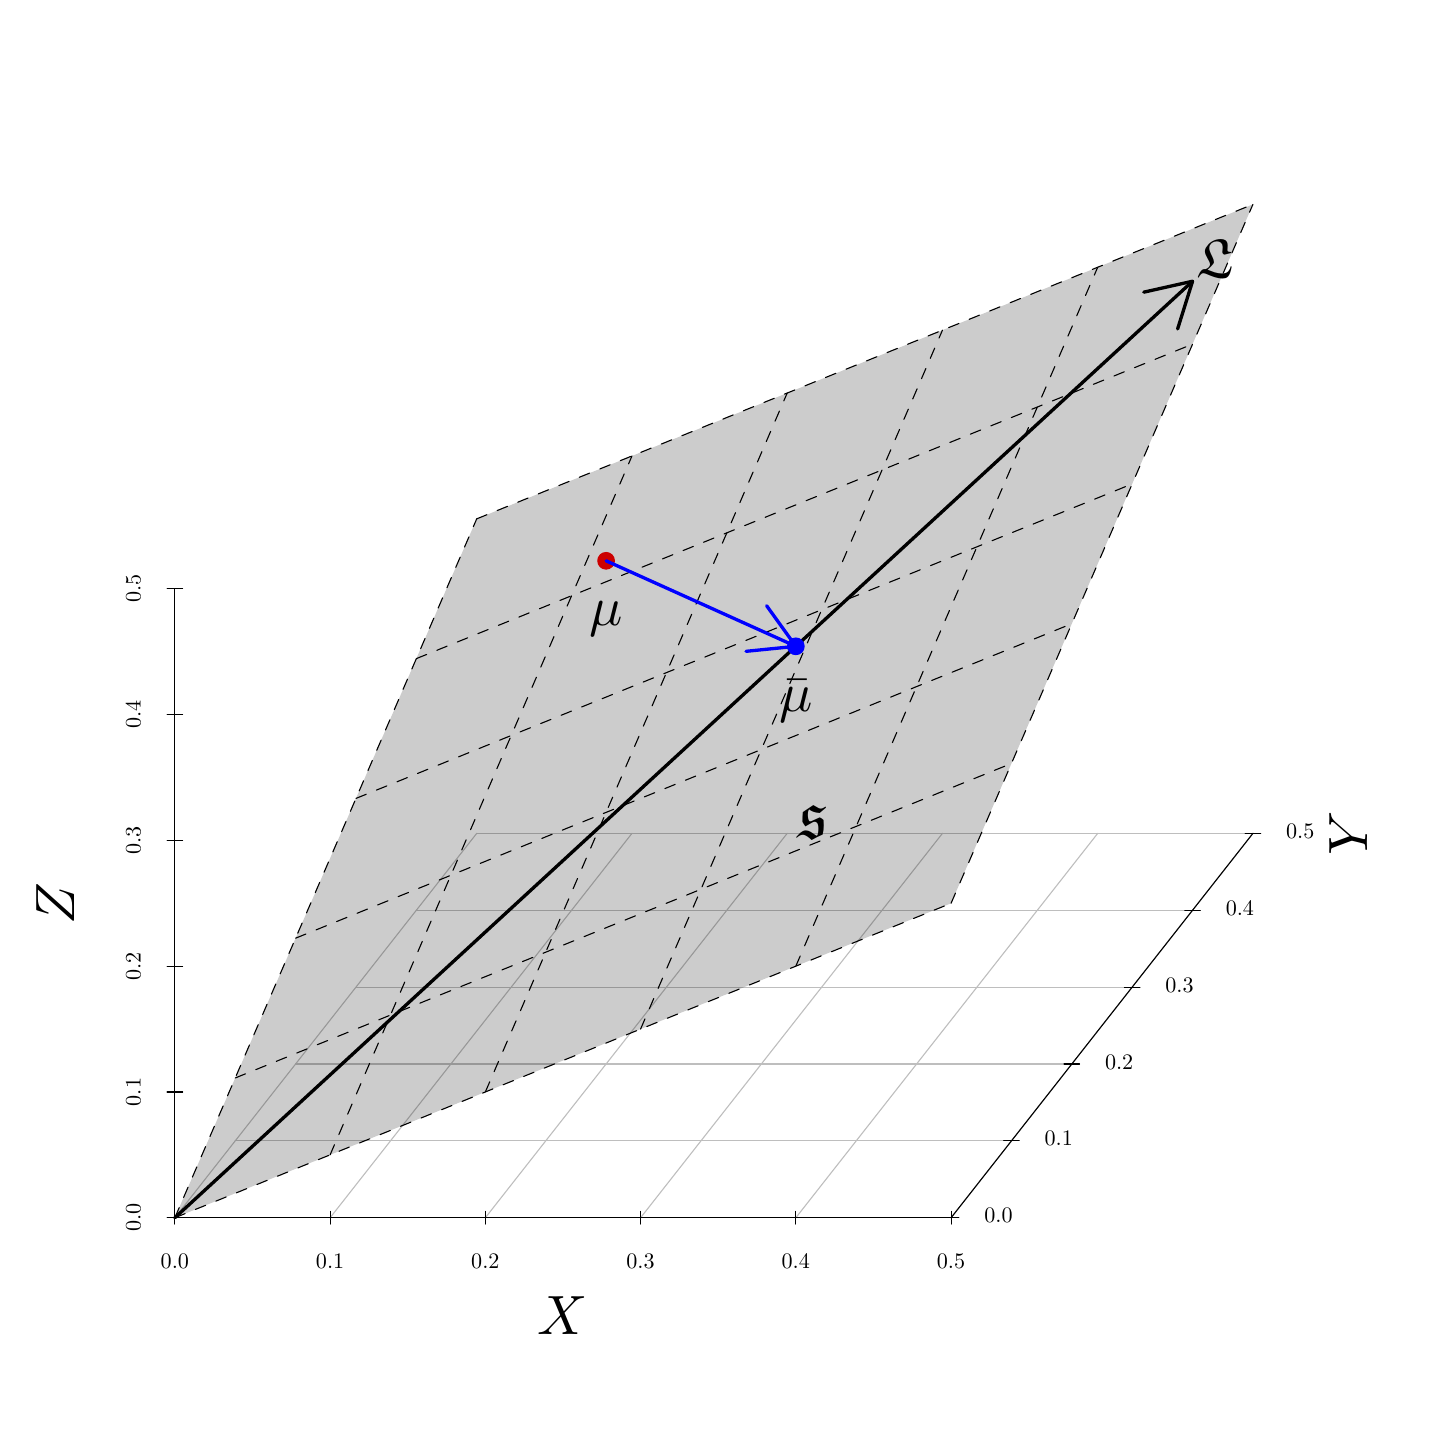
\begin{tikzpicture}[x=1pt,y=1pt]
\definecolor{fillColor}{RGB}{255,255,255}
\path[use as bounding box,fill=fillColor,fill opacity=0.00] (0,0) rectangle (505.89,505.89);
\begin{scope}
\path[clip] ( 37.20, 61.20) rectangle (468.69,456.69);
\definecolor{drawColor}{RGB}{190,190,190}

\path[draw=drawColor,line width= 0.4pt,line join=round,line cap=round] ( 53.18, 75.85) -- (162.26,214.75);

\path[draw=drawColor,line width= 0.4pt,line join=round,line cap=round] (109.28, 75.85) -- (218.36,214.75);

\path[draw=drawColor,line width= 0.4pt,line join=round,line cap=round] (165.38, 75.85) -- (274.45,214.75);

\path[draw=drawColor,line width= 0.4pt,line join=round,line cap=round] (221.47, 75.85) -- (330.55,214.75);

\path[draw=drawColor,line width= 0.4pt,line join=round,line cap=round] (277.57, 75.85) -- (386.65,214.75);

\path[draw=drawColor,line width= 0.4pt,line join=round,line cap=round] (333.67, 75.85) -- (442.74,214.75);

\path[draw=drawColor,line width= 0.4pt,line join=round,line cap=round] ( 53.18, 75.85) -- (333.67, 75.85);

\path[draw=drawColor,line width= 0.4pt,line join=round,line cap=round] ( 75.00,103.63) -- (355.48,103.63);

\path[draw=drawColor,line width= 0.4pt,line join=round,line cap=round] ( 96.81,131.41) -- (377.30,131.41);

\path[draw=drawColor,line width= 0.4pt,line join=round,line cap=round] (118.63,159.19) -- (399.11,159.19);

\path[draw=drawColor,line width= 0.4pt,line join=round,line cap=round] (140.44,186.97) -- (420.93,186.97);

\path[draw=drawColor,line width= 0.4pt,line join=round,line cap=round] (162.26,214.75) -- (442.74,214.75);
\definecolor{drawColor}{RGB}{0,0,0}

\path[draw=drawColor,line width= 0.4pt,line join=round,line cap=round] (330.86, 75.85) -- (336.47, 75.85);

\path[draw=drawColor,line width= 0.4pt,line join=round,line cap=round] (352.68,103.63) -- (358.29,103.63);

\path[draw=drawColor,line width= 0.4pt,line join=round,line cap=round] (374.49,131.41) -- (380.10,131.41);

\path[draw=drawColor,line width= 0.4pt,line join=round,line cap=round] (396.31,159.19) -- (401.92,159.19);

\path[draw=drawColor,line width= 0.4pt,line join=round,line cap=round] (418.12,186.97) -- (423.73,186.97);

\path[draw=drawColor,line width= 0.4pt,line join=round,line cap=round] (439.94,214.75) -- (445.55,214.75);

\path[draw=drawColor,line width= 0.4pt,line join=round,line cap=round] ( 53.18, 73.57) -- ( 53.18, 78.12);

\path[draw=drawColor,line width= 0.4pt,line join=round,line cap=round] (109.28, 73.57) -- (109.28, 78.12);

\path[draw=drawColor,line width= 0.4pt,line join=round,line cap=round] (165.38, 73.57) -- (165.38, 78.12);

\path[draw=drawColor,line width= 0.4pt,line join=round,line cap=round] (221.47, 73.57) -- (221.47, 78.12);

\path[draw=drawColor,line width= 0.4pt,line join=round,line cap=round] (277.57, 73.57) -- (277.57, 78.12);

\path[draw=drawColor,line width= 0.4pt,line join=round,line cap=round] (333.67, 73.57) -- (333.67, 78.12);

\path[draw=drawColor,line width= 0.4pt,line join=round,line cap=round] ( 50.38, 75.85) -- ( 55.99, 75.85);

\path[draw=drawColor,line width= 0.4pt,line join=round,line cap=round] ( 50.38,121.31) -- ( 55.99,121.31);

\path[draw=drawColor,line width= 0.4pt,line join=round,line cap=round] ( 50.38,166.77) -- ( 55.99,166.77);

\path[draw=drawColor,line width= 0.4pt,line join=round,line cap=round] ( 50.38,212.22) -- ( 55.99,212.22);

\path[draw=drawColor,line width= 0.4pt,line join=round,line cap=round] ( 50.38,257.68) -- ( 55.99,257.68);

\path[draw=drawColor,line width= 0.4pt,line join=round,line cap=round] ( 50.38,303.14) -- ( 55.99,303.14);
\end{scope}
\begin{scope}
\path[clip] (  0.00,  0.00) rectangle (505.89,505.89);
\definecolor{drawColor}{RGB}{0,0,0}

\node[text=drawColor,anchor=base,inner sep=0pt, outer sep=0pt, scale=  0.80] at ( 53.18, 57.60) {0.0};

\node[text=drawColor,anchor=base,inner sep=0pt, outer sep=0pt, scale=  0.80] at (109.28, 57.60) {0.1};

\node[text=drawColor,anchor=base,inner sep=0pt, outer sep=0pt, scale=  0.80] at (165.38, 57.60) {0.2};

\node[text=drawColor,anchor=base,inner sep=0pt, outer sep=0pt, scale=  0.80] at (221.47, 57.60) {0.3};

\node[text=drawColor,anchor=base,inner sep=0pt, outer sep=0pt, scale=  0.80] at (277.57, 57.60) {0.4};

\node[text=drawColor,anchor=base,inner sep=0pt, outer sep=0pt, scale=  0.80] at (333.67, 57.60) {0.5};

\node[text=drawColor,rotate= 90.00,anchor=base,inner sep=0pt, outer sep=0pt, scale=  0.80] at ( 40.80, 75.85) {0.0};

\node[text=drawColor,rotate= 90.00,anchor=base,inner sep=0pt, outer sep=0pt, scale=  0.80] at ( 40.80,121.31) {0.1};

\node[text=drawColor,rotate= 90.00,anchor=base,inner sep=0pt, outer sep=0pt, scale=  0.80] at ( 40.80,166.77) {0.2};

\node[text=drawColor,rotate= 90.00,anchor=base,inner sep=0pt, outer sep=0pt, scale=  0.80] at ( 40.80,212.22) {0.3};

\node[text=drawColor,rotate= 90.00,anchor=base,inner sep=0pt, outer sep=0pt, scale=  0.80] at ( 40.80,257.68) {0.4};

\node[text=drawColor,rotate= 90.00,anchor=base,inner sep=0pt, outer sep=0pt, scale=  0.80] at ( 40.80,303.14) {0.5};
\end{scope}
\begin{scope}
\path[clip] ( 37.20, 61.20) rectangle (468.69,456.69);
\definecolor{drawColor}{RGB}{0,0,0}

\node[text=drawColor,anchor=base west,inner sep=0pt, outer sep=0pt, scale=  0.80] at (345.67, 74.01) {0.0};

\node[text=drawColor,anchor=base west,inner sep=0pt, outer sep=0pt, scale=  0.80] at (367.48,101.79) {0.1};

\node[text=drawColor,anchor=base west,inner sep=0pt, outer sep=0pt, scale=  0.80] at (389.30,129.57) {0.2};

\node[text=drawColor,anchor=base west,inner sep=0pt, outer sep=0pt, scale=  0.80] at (411.11,157.35) {0.3};

\node[text=drawColor,anchor=base west,inner sep=0pt, outer sep=0pt, scale=  0.80] at (432.93,185.13) {0.4};

\node[text=drawColor,anchor=base west,inner sep=0pt, outer sep=0pt, scale=  0.80] at (454.74,212.91) {0.5};

\path[draw=drawColor,line width= 0.4pt,line join=round,line cap=round] ( 53.18, 75.85) --
	(333.67, 75.85);
\end{scope}
\begin{scope}
\path[clip] (  0.00,  0.00) rectangle (505.89,505.89);
\definecolor{drawColor}{RGB}{0,0,0}

\node[text=drawColor,anchor=base,inner sep=0pt, outer sep=0pt, scale=  2.00] at (193.42, 33.60) {$X$};
\end{scope}
\begin{scope}
\path[clip] ( 37.20, 61.20) rectangle (468.69,456.69);
\definecolor{drawColor}{RGB}{0,0,0}

\path[draw=drawColor,line width= 0.4pt,line join=round,line cap=round] (333.67, 75.85) --
	(442.74,214.75);
\end{scope}
\begin{scope}
\path[clip] (  0.00,  0.00) rectangle (505.89,505.89);
\definecolor{drawColor}{RGB}{0,0,0}

\node[text=drawColor,rotate= 90.00,anchor=base,inner sep=0pt, outer sep=0pt, scale=  2.00] at (484.29,214.75) {$Y$};
\end{scope}
\begin{scope}
\path[clip] ( 37.20, 61.20) rectangle (468.69,456.69);
\definecolor{drawColor}{RGB}{0,0,0}

\path[draw=drawColor,line width= 0.4pt,line join=round,line cap=round] ( 53.18, 75.85) --
	( 53.18,303.14);
\end{scope}
\begin{scope}
\path[clip] (  0.00,  0.00) rectangle (505.89,505.89);
\definecolor{drawColor}{RGB}{0,0,0}

\node[text=drawColor,rotate= 90.00,anchor=base,inner sep=0pt, outer sep=0pt, scale=  2.00] at ( 16.80,189.49) {$Z$};
\end{scope}
\begin{scope}
\path[clip] ( 37.20, 61.20) rectangle (468.69,456.69);
\definecolor{drawColor}{RGB}{255,0,0}
\definecolor{fillColor}{RGB}{255,0,0}

\path[draw=drawColor,line width= 0.4pt,line join=round,line cap=round,fill=fillColor] (209.01,313.24) circle (  3.00);
\definecolor{fillColor}{RGB}{0,0,0}

\path[fill=fillColor,fill opacity=0.20] ( 53.18, 75.85) --
	(162.26,328.40) --
	(442.74,442.04) --
	(333.67,189.49) --
	cycle;
\definecolor{drawColor}{RGB}{0,0,0}

\path[draw=drawColor,line width= 0.4pt,dash pattern=on 4pt off 4pt ,line join=round,line cap=round] ( 53.18, 75.85) -- (162.26,328.40);

\path[draw=drawColor,line width= 0.4pt,dash pattern=on 4pt off 4pt ,line join=round,line cap=round] (109.28, 98.58) -- (218.36,351.12);

\path[draw=drawColor,line width= 0.4pt,dash pattern=on 4pt off 4pt ,line join=round,line cap=round] (165.38,121.31) -- (274.45,373.85);

\path[draw=drawColor,line width= 0.4pt,dash pattern=on 4pt off 4pt ,line join=round,line cap=round] (221.47,144.04) -- (330.55,396.58);

\path[draw=drawColor,line width= 0.4pt,dash pattern=on 4pt off 4pt ,line join=round,line cap=round] (277.57,166.77) -- (386.65,419.31);

\path[draw=drawColor,line width= 0.4pt,dash pattern=on 4pt off 4pt ,line join=round,line cap=round] (333.67,189.49) -- (442.74,442.04);

\path[draw=drawColor,line width= 0.4pt,dash pattern=on 4pt off 4pt ,line join=round,line cap=round] ( 53.18, 75.85) -- (333.67,189.49);

\path[draw=drawColor,line width= 0.4pt,dash pattern=on 4pt off 4pt ,line join=round,line cap=round] ( 75.00,126.36) -- (355.48,240.00);

\path[draw=drawColor,line width= 0.4pt,dash pattern=on 4pt off 4pt ,line join=round,line cap=round] ( 96.81,176.87) -- (377.30,290.51);

\path[draw=drawColor,line width= 0.4pt,dash pattern=on 4pt off 4pt ,line join=round,line cap=round] (118.63,227.38) -- (399.11,341.02);

\path[draw=drawColor,line width= 0.4pt,dash pattern=on 4pt off 4pt ,line join=round,line cap=round] (140.44,277.89) -- (420.93,391.53);

\path[draw=drawColor,line width= 0.4pt,dash pattern=on 4pt off 4pt ,line join=round,line cap=round] (162.26,328.40) -- (442.74,442.04);

\path[draw=drawColor,line width= 1.2pt,line join=round,line cap=round] ( 53.18, 75.85) -- (420.93,414.26);

\path[draw=drawColor,line width= 1.2pt,line join=round,line cap=round] (415.53,397.02) --
	(420.93,414.26) --
	(403.30,410.31);
\definecolor{drawColor}{RGB}{0,0,255}
\definecolor{fillColor}{RGB}{0,0,255}

\path[draw=drawColor,line width= 0.4pt,line join=round,line cap=round,fill=fillColor] (277.57,282.34) circle (  3.00);

\path[draw=drawColor,line width= 1.2pt,line join=round,line cap=round] (209.01,313.24) -- (277.57,282.34);

\path[draw=drawColor,line width= 1.2pt,line join=round,line cap=round] (259.59,280.53) --
	(277.57,282.34) --
	(267.02,297.00);
\definecolor{drawColor}{RGB}{0,0,0}

\node[text=drawColor,anchor=base west,inner sep=0pt, outer sep=0pt, scale=  2.00] at (422.26,415.64) {{$\mathfrak{L}$}};

\node[text=drawColor,anchor=base,inner sep=0pt, outer sep=0pt, scale=  2.00] at (209.01,289.76) {{$\mu$}};

\node[text=drawColor,anchor=base,inner sep=0pt, outer sep=0pt, scale=  2.00] at (277.57,258.86) {{$\bar{\mu}$}};

\node[text=drawColor,anchor=base west,inner sep=0pt, outer sep=0pt, scale=  1.00] at (278.67,212.91) {{\Huge $\mathfrak{s}$}};
\end{scope}
\end{tikzpicture}

  }
  \caption{$\mathfrak{L}$ is a linear subspace of the coherent subspace $\mathfrak{s}$. If a projection is onto $\mathfrak{L}$ instead of $\mathfrak{s}$, then $\bm{\mu} \in \mathfrak{s}$ will be moved to $\bm{\mu}^* \in \mathfrak{L}$.}\label{fig:Schematic_3D}
\end{figure}

Finally, it is often stated that an assumption required to prove the unbiasedness preserving property is that $\bm{S}\bm{G}\bm{S}=\bm{S}$ or alternatively that $\bm{G}\bm{S}=\bm{I}$. Both of these conditions are equivalent to assuming that $\bm{S}\bm{G}$ is a projection matrix (see Section~\ref{app:projection-proof} in Appendix A for a proof). {\color{blue}{Despite this connection,}} problems arise when viewing the preservation of unbiasedness through the prism of imposing the constraint $\bm{G}\bm{S}=\bm{I}$. This thinking suggests that a way to deal with biased forecasts is to select $\bm{G}$ in an unconstrained manner. Equipped with a geometric understanding of the problem, we would advise against this approach. The constraint $\bm{G}\bm{S}=\bm{I}$ is not just about bias. Dropping the constraint compromises all of the attractive properties of projections. It also opens the door to reconciliation methods that change already coherent base forecasts, which suggests an increase in the variability of the forecasts. This seems particularly perverse when the motivation for using a biased method in the first place is to reduce variance.

\subsection{Bias correction}

Our own solution to dealing with biased forecasts is to bias correct \emph{before} reconciliation. In many cases the method for bias correction will be context specific. For instance, in our empirical study in Section~\ref{sec:EmpStudy} we consider a scenario where {\color{blue} data are modelled after} taking either a log transformation or a Box-Cox transformation. {\color{blue} Since linear constraints that hold on the original scale do not hold for the transformed series, back-transforming to the original scale is necessary.  Since this step induces a bias we propose to bias correct after this back-transformation step, but before reconciliation.}  In the well-known case {\color{blue} of the Box-Cox transformation} a number of bias correction methods exist based on Taylor expansions.

Alternatively, a more general purpose approach to bias correction is to simply estimate the bias by taking the sample mean of $\bm{y}_{t+h}-\hat{\bm{y}}_{t+h|t}$ for all $t+h$ in the training sample. This can then be subtracted from future forecasts. As stated in the discussion of MinT, in-sample errors are already used to estimate the optimal direction of projection. As such it may be possible to use the same errors to bias correct. Geometrically, the intuition is simple. In panel~(a) of Figure~\ref{fig:OthogonalVSOblique_projection}, the orange points are centered around the origin as would be expected from an unbiased forecast. If forecasts are biased, then errors should simply be translated until they are centered at the origin. Nonetheless there are also a number of pitfalls to such an approach. First, for the very construction we consider, where bias is induced by taking a log or Box Cox transformation, bias should be corrected by a multiplicative rather than an additive factor. Second, if in-sample errors are non-stationary due to model misspecification or structural breaks, then the proposed method for bias correction may break down.

\section{Empirical study}\label{sec:EmpStudy}

Using an empirical application to forecast Australian domestic tourism flows, we illustrate the usefulness of projection-based reconciliation in practice. Previous studies have found that reconciliation improves point forecast accuracy in domestic tourism flows for Australia \citep[see for example][]{Athanasopoulos2009, Hyndman2011,WicEtAl2019}. Our motivation in this study is twofold. First, we demonstrate the implications of Theorem~\ref{th:distred} {\color{blue} and Theorem~\ref{th:gmint}} by comparing reconciled and base forecasts. In contrast to previous studies, we consider individual periods {\color{blue} as well as} compute averages over a rolling window. Second, we demonstrate how the bias correction methods discussed in the previous section along with the projection-based reconciliation help to improve forecast accuracy.

\subsection{Data}

We consider ``overnight trips'' across Australia as a measure of domestic tourism flows. The data are provided by the National Visitor Survey and are collected through telephone interviews from an annual sample of $120,000$ Australian residents aged $15$ years or more. We disaggregate tourism flows into 7 states, 27 zones and 75 regions forming a natural geographical hierarchy that is of interest to tourism operators and policy makers amongst others. Hence, there are $110$ series across the hierarchy with $75$ bottom-level series. More information about the series and the geographical hierarchy is presented in Table~\ref{table:A1} in Appendix B\@. The data span the period January 1998 to December 2017, which gives a total of $240$ observations per series.

Figure~\ref{fig:Total_TSplots} shows time, sub-series and seasonal plots of the aggregate overnight trips. As is usual with tourism data, these show a strong seasonal pattern with peaks observed every January corresponding to the summer vacation season in Australia. There are also some lower peaks observed in April, July and October corresponding to school term breaks. On the other hand, the month with the least overnight trips is February indicating that people travel least for the month following their summer vacation. The time plot also shows a pronounced upward trend starting from around 2010 to the end of the sample, with flows being fairly flat from the beginning of the sample and a slight downward trend during 2004--2010.

The top panel of Figure~\ref{fig:States_Zones_Regs_TSplots} shows time plots for the seven states, hence the first level of the geographical hierarchy. The panels below show some selected series from the second-level zones and the bottom-level regions. The plots display the diversity of time series features, within but also between levels. For example, noticeable at the first level is the asynchronous seasonal pattern between the Northern Territory and the other states. For the Northern Territory the high tourist season occurs during June-August with July being the peak, while the low season is during December-February. This reflects the tropical climate of the Northern Territory, with Australians mostly visiting the North during its dry winter-season rather than the wet summer season. Noticeable as we move to the lower levels is the variation in the signal-to-noise ratio, with the regional bottom-level series being much noisier compared to the series from levels above. This of course highlights the importance of modelling series at all levels without any loss of valuable information. We should note here that we observed an anomalous (extremely high) observation for `Adelaide Hills' for December 2002. We replaced this observation with the average overnight trips on December 2001 and December 2003 for the same destination.

\begin{figure}
  \centering
  \small
  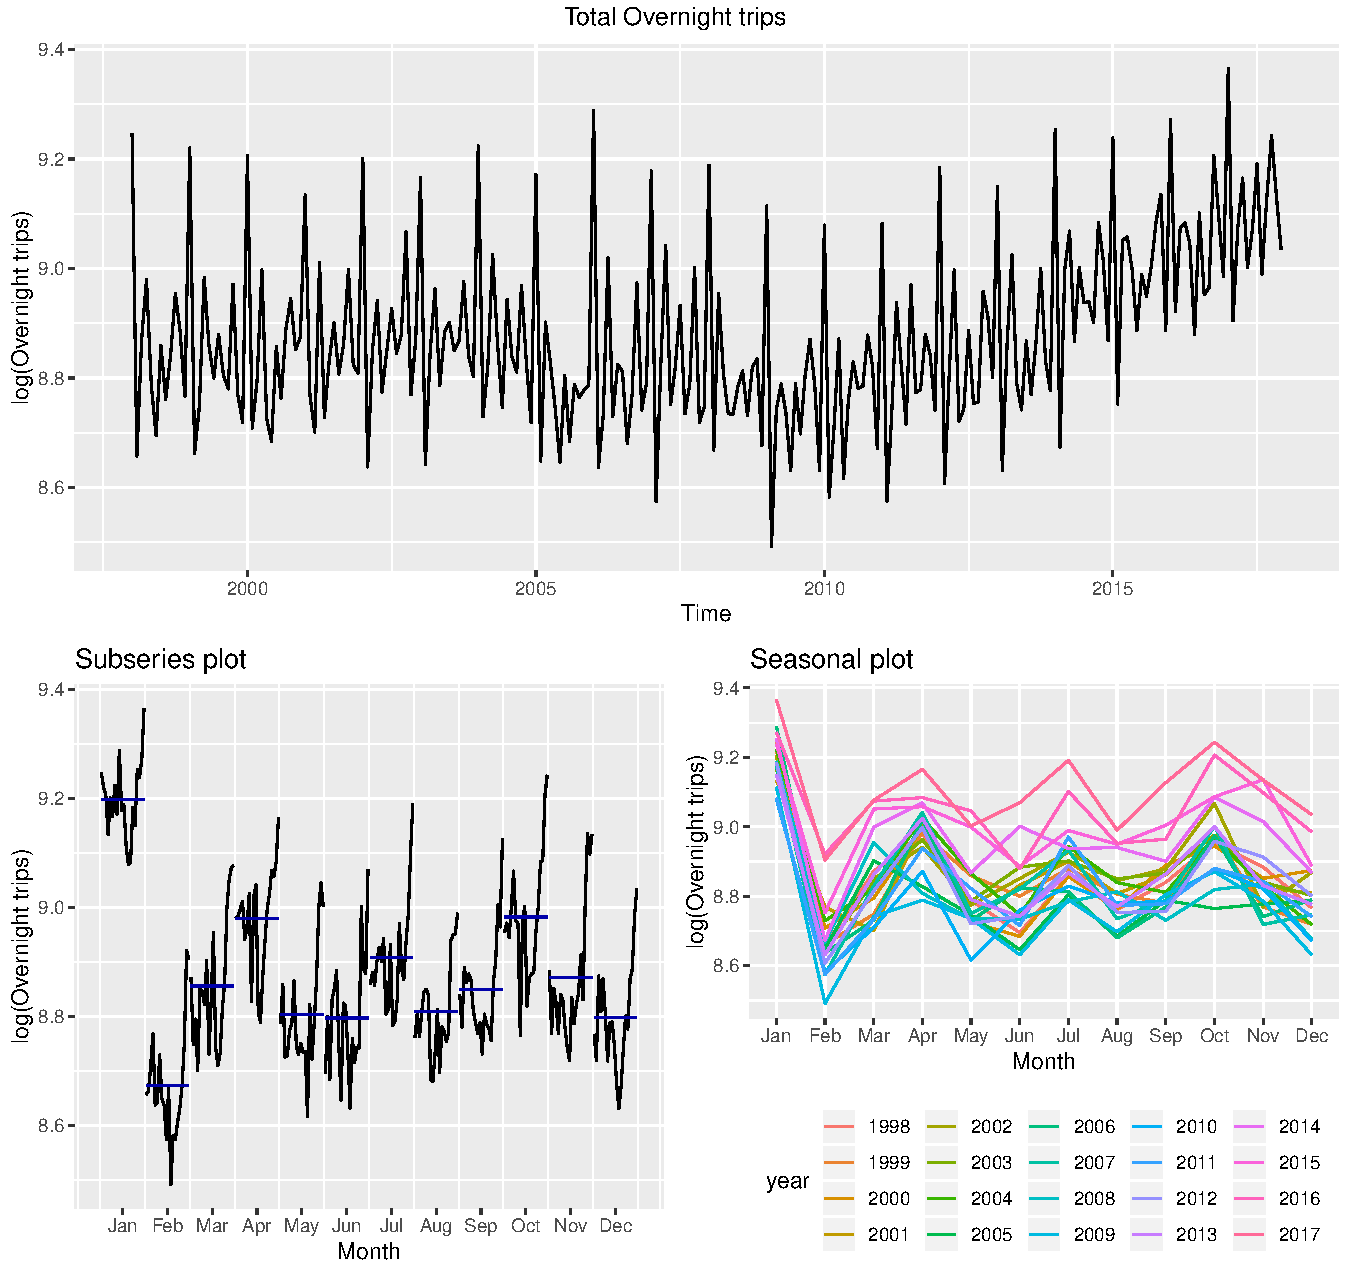
\includegraphics[width = \textwidth]{Empirical-results/TS-plots/Total_TSplots.pdf}
  \caption{Total domestic overnight trips (in logs) for Australia from January 1998 to December 2017. The top-panel shows a time plot; the bottom-left panel a sub-series plot for each month; the bottom-right panel shows a seasonal plot coloured by year.}\label{fig:Total_TSplots}
\end{figure}

\begin{figure}
  \centering
  \small
  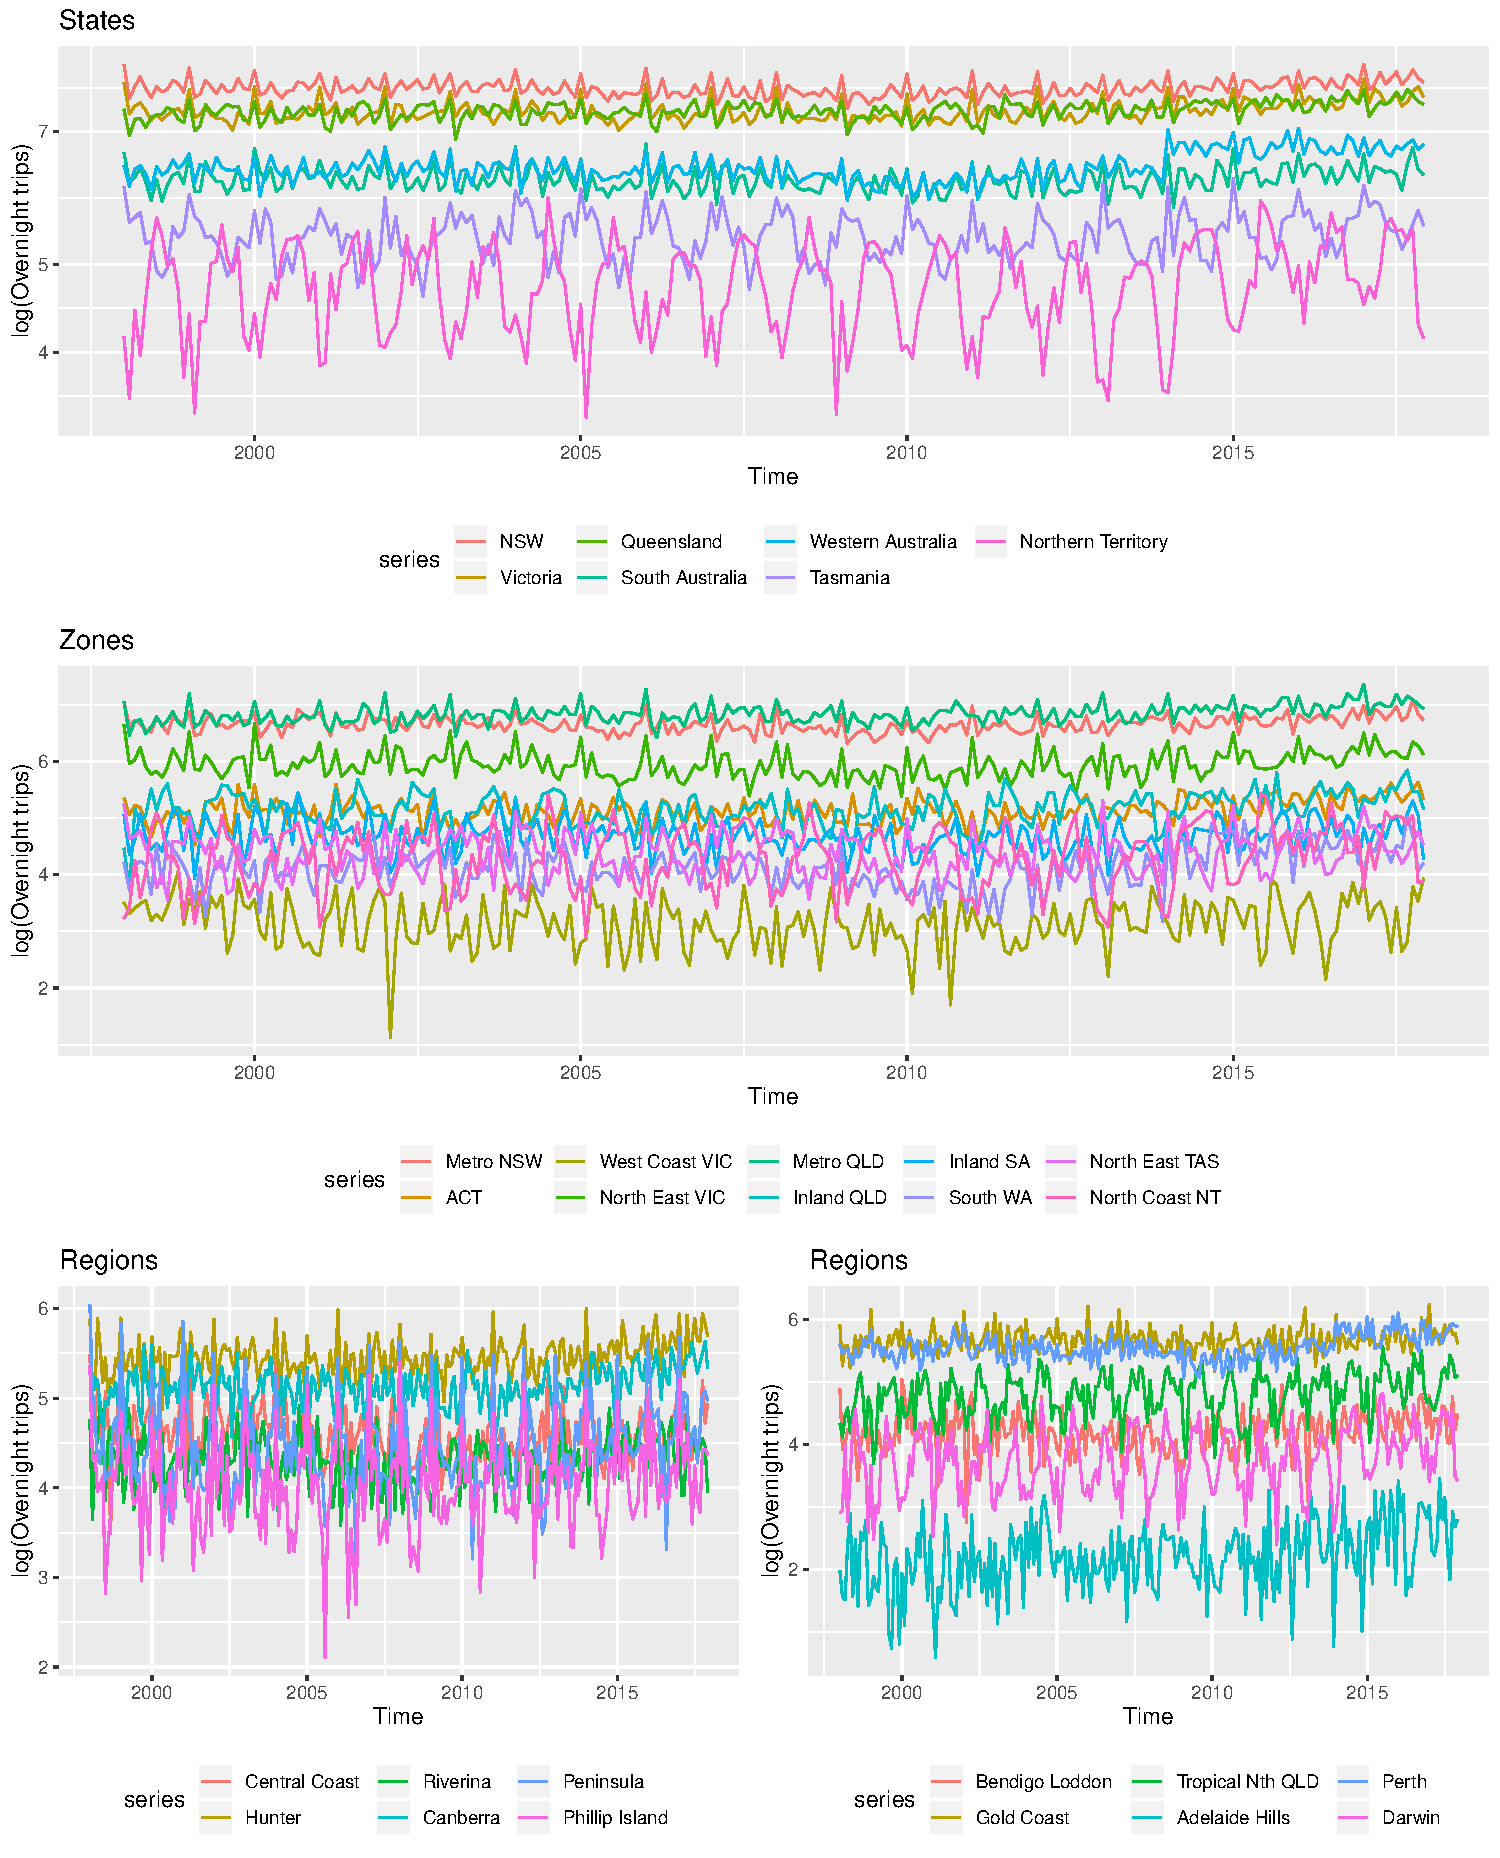
\includegraphics[width= .95\textwidth]{Empirical-results/TS-plots/States_Zones_Regs_TSplots1.pdf}
  \caption{Time plot of overnight trips for some selected series from different disaggregate levels of the hierarchy. All values are presented in log scale. To avoid impact from the zero values we added a constant 1 to all observations}\label{fig:States_Zones_Regs_TSplots}
\end{figure}

\clearpage

{\color{red} I've done a clear page here so we can see the flow better. We will remove this}

\subsection{Comparison to Base Forecasts}\label{sec:comparebase}

To demonstrate the implications of Theorem~\ref{th:distred} we consider the improvement of different reconciliation methods over base forecasts {\color{blue} using different loss functions}. For each series the ARIMA model minimising AICc is chosen using the \verb|auto.arima()| function in the \verb|forecast| package. Using these fitted models, base forecasts are produced for $h=1$ to $6$-steps ahead for each series in the hierarchy. This is first carried out with a training sample of $100$ observations, i.e., Jan-$1998$ to Apr-$2006$. The training window is then rolled forward one observation at a time until the end of the sample. This generates $140~1$-step-ahead, $139~2$-steps-ahead through to $135~6$-steps-ahead forecasts available for forecast evaluation.

{\color{red} I think the flow here is a bit confusing. I see that we need to talk about the loss functions before the reconciliation methods because of Spend-WLS. I suggest the following. We first introduce the three typical reconciliation methods - OLS, Structural-WLS and MinT and move the paragraph that introduces these above. Then when we introduce the loss functions we introduce in the second paragraph, starting ``The second choice'' Spend-WLS. I've re-written 5.2 based on this thought and called it -George in the end. See what do you think? Please delete appropriately.}

{\color{blue} For each replication {\color{red} and for method $q$,- I don't think we need this here - $q$ is defined over the page} we compute three loss functions.  The first is the total squared error (TSE), computed as
	\begin{equation}
	\label{eq:tse}
	\textrm{TSE}^{q}_t=\sum\limits_{i=1}^n(y_{i,t}-\tilde{y}^{(q)}_{i,t})^2\,,
	\end{equation}
	where $\tilde{y}^{(q)}$ is the reconciled forecast using method $q$ for series $i$ and replication $t$.
This loss function is the square of the usual Euclidean distance described in Section~\ref{sec:orthogonal}. We also consider loss functions based on a squared generalised Euclidean distance of the form
\begin{equation*}
	\textrm{WSE}^{q}_t=\sum\limits_{i=1}^n \left(w_i (y_{i,t}-\tilde{y}^{(q)}_{i,t})\right)^2\,,
	\end{equation*}
	We consider two choices of weights.  The first is the inverse of the number of bottom-level series included in forming a specific aggregate.  For example, for all bottom-level series this weight is 1, whereas for the top-level series this is 1/75.  The idea is to ensure top-level series, which are on a much larger scale, do not dominate the forecast evaluation metric.  Using these weights in WLS reconciliation is equivalent to what \cite{AthEtAl2017} refer to as \textit{structural scaling}.  As such we refer to WLS based on these weights as `Structural-WLS' and the loss function based on these weights as `Structural-WSE'.
	
	The second choice of weights is motivated by our empirical example.  In addition to visitor numbers per region, we also have access to data on average spend per region.  In some settings, it may be desirable to have greater forecast accuracy in regions where tourists spend more.  By using average spend per region as weights, the error metric (and transformed space associated with this metric) can be interpreted in terms of revenue measured in dollars rather than raw tourist numbers. We refer to WLS based on these weights as `Spend-WLS' and the loss function based on these weights as `Spend-WSE'.
}

After obtaining the base forecasts these are reconciled using four different projection methods: OLS, {\color{blue} Structural-WLS, Spend-WLS  and MinT.   For MinT, the shrinkage estimator of \cite{Schafer2005} is used to estimate  $\bm{\Sigma}$. The estimate is $\tau\text{diag}(\hat{\bm{\Sigma}}) + (1-\tau)\hat{\bm{\Sigma}}$  where $\hat{\bm{\Sigma}}$ is the sample estimate of the variance covariance matrix of the in-sample, one-step ahead forecast errors and,
	\begin{equation*}
	\tau = \frac{\sum_{i \neq j}\hat{\var}(\hat{\sigma}_{ij})}{\sum_{i \neq j}{\hat{\sigma}}^2_{ij}}\,,
	\end{equation*}
	where $\hat{\sigma}_{ij}$ denotes the $(i,j)$th element of $\hat{\bm{\Sigma}}$. }

\clearpage
\subsection*{Comparison to Base Forecasts - George}\label{sec:comparebase}

To demonstrate the implications of Theorem~\ref{th:distred} we consider the improvement of different reconciliation methods over base forecasts {\color{blue} using different loss functions}. For each series the ARIMA model minimising AICc is chosen using the \verb|auto.arima()| function in the \verb|forecast| package. Using these fitted models, base forecasts are produced for $h=1$ to $6$-steps ahead for each series in the hierarchy. This is first carried out with a training sample of $100$ observations, i.e., Jan-$1998$ to Apr-$2006$. The training window is then rolled forward one observation at a time until the end of the sample. This generates $140~1$-step-ahead, $139~2$-steps-ahead through to $135~6$-steps-ahead forecasts available for forecast evaluation.

After obtaining the base forecasts these are reconciled using various projection methods. In particular: OLS reconciliation; WLS reconciliation using structural scaling introduced by \cite{AthEtAl2017} which we refer to as Structural-WLS; and MinT using the shrinkage estimator of \cite{Schafer2005} to estimate  $\bm{\Sigma}$. The estimate is $\tau\text{diag}(\hat{\bm{\Sigma}}) + (1-\tau)\hat{\bm{\Sigma}}$  where $\hat{\bm{\Sigma}}$ is the sample estimate of the variance covariance matrix of the in-sample, one-step ahead forecast errors and,
	\begin{equation*}
	\tau = \frac{\sum_{i \neq j}\hat{\var}(\hat{\sigma}_{ij})}{\sum_{i \neq j}{\hat{\sigma}}^2_{ij}}\,,
	\end{equation*}
	where $\hat{\sigma}_{ij}$ denotes the $(i,j)$th element of $\hat{\bm{\Sigma}}$. 

{\color{blue} For each method we compute three loss functions.  The first is the total squared error (TSE), computed as
	\begin{equation}
	\label{eq:tse}
	\textrm{TSE}^{q}_t=\sum\limits_{i=1}^n(y_{i,t}-\tilde{y}^{(q)}_{i,t})^2\,,
	\end{equation}
	where $\tilde{y}^{(q)}$ is the reconciled forecast using method $q$ for series $i$ and replication $t$.
This loss function is the square of the usual Euclidean distance described in Section~\ref{sec:orthogonal}. We also consider loss functions based on a squared generalised Euclidean distance of the form
\begin{equation*}
	\textrm{WSE}^{q}_t=\sum\limits_{i=1}^n \left(w_i (y_{i,t}-\tilde{y}^{(q)}_{i,t})\right)^2\,,
	\end{equation*}
	We consider two choices of weights.  The first is the inverse of the number of bottom-level series included in forming a specific aggregate.  For example, for all bottom-level series this weight is 1, whereas for the top-level series this is 1/75.  The idea is to ensure top-level series, which are on a much larger scale, do not dominate the forecast evaluation metric.  These are the weights used in the Structural-WLS reconciliation approach introduced in the previous paragraph. As such we refer to the loss function based on these weights as `Structural-WSE'.
	
	The second choice of weights is motivated by our empirical example.  In addition to visitor numbers per region, we also have access to data on average spend per region.  In some settings, it may be desirable to have greater forecast accuracy in regions where tourists spend more.  By using average spend per region as weights, the error metric (and transformed space associated with this metric) can be interpreted in terms of revenue measured in dollars rather than raw tourist numbers. Using these weights we introduce an alternative WLS reconciliation approach which we refer to as `Spend-WLS'. Correspondingly we refer to the loss function based on these weights as `Spend-WSE'.
}

{\color{red} My rewrite of 5.2 ends here}

{\color{blue} For each replication we compute the ratio of the loss of each alternative reconciliation method to the loss of base forecasts. A value less than 1 indicates that a reconciliation method has a lower relative error than the base forecast for that replication, while a value greater than 1 indicates the opposite. The boxplots in Figure~\ref{fig:BaseVSRecon_Fc} summarise the distribution of these ratios over each rolling window. We only present the results for $h=1$, but the results and conclusions that follow are almost identical for the other longer forecast horizons. We do not present these here to save space but they are available {\color{red} in an online supplement.}

For TSE, relative loss is always less than 1 only for OLS reconciliation, for Structural-WSE the same is only true for Structural-WLS and for Spend-WSE the same is only true for Spend-WLS.  Therefore, Figure~\ref{fig:BaseVSRecon_Fc} demonstrates that a reconciliation method is guaranteed to improve upon base forecasts only when the $\bm{W}$ used in the loss function and reconciliation coincide.  This is precisely what Theorem~\ref{th:distred} and Theorem~\ref{th:gdistred} would predict.  On the other hand, for every loss function, MinT will perform worse than base for some realisations.  For Theorem~\ref{th:gdistred} to hold for MinT, the loss function would need to set $\bm{W}=\bm{\Sigma}^{-1}$. Since the estimate of ${\bm\Sigma}$ will change with each replication we do not believe this is a sensible loss function to use.


}

%As the theory predicts, OLS reconciliation always leads to an improvement relative to base forecasts. The entire boxplot for OLS reconciliation is above zero. This is not the case for MinT and WLS which for some windows generate forecasts less accurate than the base forecasts. The boxplots also demonstrate that OLS reconciliation is more stable than MinT and WLS reconciliation, a result not entirely unsurprising since the latter two methods require estimation of a $\bm{W}$ matrix which in practice is not trivial. Nonetheless when averaging over the entire rolling window the MinT estimator performs best on average, which is again precisely what the theorem proved in \citet{WicEtAl2019} would suggest. The average MSE values across the entire rolling window of 140 replications are shown in Table \ref{tab:AveraveDifferences}.

\begin{figure}[!hbt]
    \centering
    \small
    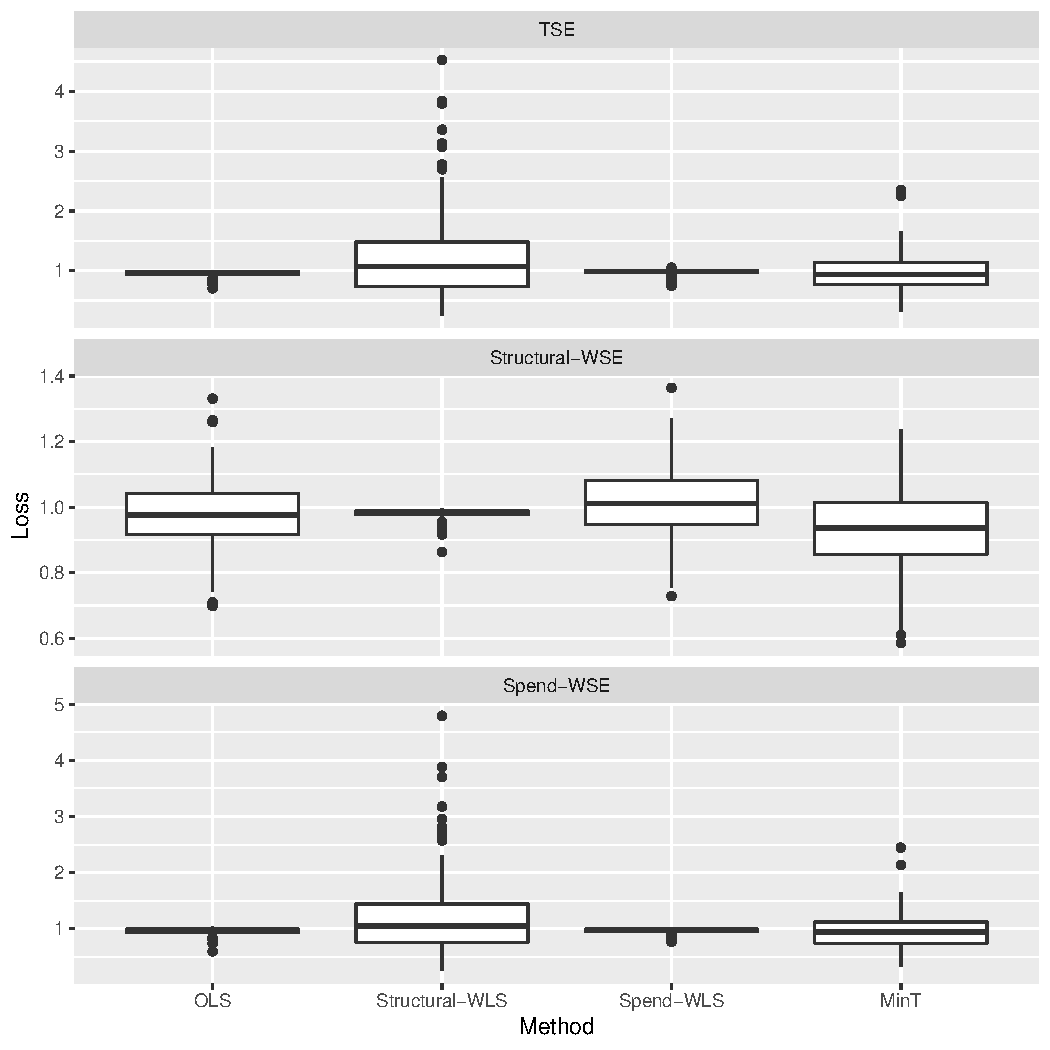
\includegraphics[width = \textwidth, height=14cm]{Figs/lossboxplots_1.pdf}
    \caption{{\color{blue} Ratio of loss of reconciled forecast to loss of base forecast for $h = 1$. A value less than 1 indicates that the reconciled forecasts improve upon base forecasts.  A log scale is used for the y axis.}}\label{fig:BaseVSRecon_Fc}
\end{figure}

%\begin{table}[!hbt]
%\caption {Average {MSE($\times 10^3$)} over all 140 rolling window replications for $h=1$.}\label{tab:AveraveDifferences}
%  \centering \tabcolsep=0.4cm
%  \begin{tabular}{lccccc}
%  \toprule
%          & Base & OLS & MinT & WLS & Bottom-up \\
%   MSE    & 4.31 & 4.20 & \textbf{4.16} & 4.48 & 5.28 \\
%  \bottomrule
%  \end{tabular}
%\end{table}

{\color{blue}

The advantage of MinT however is clearly seen when loss functions are averaged (an estimate of expected loss).  Table~\ref{tab:lossVmethods} reports the relative total error for each loss function. For example, for TSE the relative mean total squared error (RMTSE) is defined as
\begin{equation}
\textrm{RMTSE}^{q}=\frac{\frac{1}{140}\sum\limits_{t=1}^{140}\textrm{TSE}^{q}_t}{\frac{1}{140}\sum\limits_{t=1}^{140}\textrm{TSE}^{\textrm{Base}}_t}\,\label{eq:RTSE}
\end{equation}
where $\textrm{TSE}^{\textrm{Base}}_t$ is the total squared error of the base forecasts at replication $t$.  In contrast with what is displayed in the boxplots, here the average is taken over the replications before taking a ratio.  Table~\ref{tab:lossVmethods} shows that the average loss for MinT is lower than for all other reconciliation methods, irrespective of the loss function used.  This is precisely what would be expected from Theorem~\ref{th:gmint}. {\color{red} You said you commented on statistical significance but I cannot see it. I wonder what the Nemenyi matrix tests will look like here. Maybe these will show some stat significances worth reporting. --- Ok I see it is in the caption but the sentence needs fixing. Maybe it is best to have in the text rather than the caption.}
}

\begin{table}[ht]
	\centering
{\color{blue}	
	\begin{tabular}{lrrrrrr}
		\hline
		Loss Function & Base & Bottom-up & OLS & Structural-WLS & Spend-WLS & MinT \\
		\hline
		TSE & 1.00 & 1.22 & 0.97 & 1.13 & 0.98 & 0.96 \\
		Structural-WSE & 1.00 & 1.01 & 0.96 & 0.98 & 1.00 & 0.93 \\
		Spend-WSE & 1.00 & 1.20 & 0.97 & 1.12 & 0.98 & 0.96 \\
		\hline
    \end{tabular}
}
	\caption{{\color{blue}Means of different loss functions for 1-step ahead forecasts using different reconciliation methods in the tourism application.  All figures are reported relative to base forecasts.  The lowest mean is always provided by MinT, for Structural-WSE, the average loss for MinT is significantly than every other method.}}
	\label{tab:lossVmethods}
\end{table}


\subsection{Transformations and bias adjustment}

We first transform each series in the hierarchy using two types of transformations. Namely, we perform a log-transformation and also the more general Box-Cox transformation. A Box-Cox transformation is defined as,
\begin{equation*}\label{eq:BoxCox_transformation}
w_t = \begin{cases}
        \log(y_t)                        & \text{if}~\lambda=0;\\
        \frac{y_t^\lambda - 1}{\lambda}  & \text{otherwise}.
      \end{cases}
\end{equation*}
We first set $\lambda=0$ and hence consider only a log transformation. For the second more general Box-Cox transformation we select $\lambda$ using the ``Guerrero'' method \citep{guerrero1993time} implemented in the \verb|BoxCox.lambda()| function in the \verb|forecast| package in R \citep{Rforecast}. In order to avoid extreme and volatile transformations we restrict $\lambda \in (-0.5,2)$. As zero observations exist in some of the bottom-level series, before transforming we add a constant (more specifically $1$) to each series. This overcomes the challenge of undefined transformed values for zero observations when we specifically implement the log transformation or when $\lambda$ is selected to be zero by the ``Guerrero'' method. The constant is subtracted from the final forecasts.

After transformation we fit univariate ARIMA models to each transformed series. The \verb|auto.arima()| function in the \verb|forecast| package is used to choose the best model that minimises the AICc. Using the fitted models, forecasts are produced for $h=1$ to $12$-steps ahead for each series in the hierarchy. The same rolling window described in Section~\ref{sec:comparebase} is used here as well.

The forecasts are then back-transformed by simply reversing the Box-Cox transformation using,
\begin{equation}\label{eq:BoxCox_back-transformation}
  \hat{y}_{t+h|t} =
    \begin{cases}
      \exp({\hat{w}_{t+h|t}})                   & \text{if}~\lambda = 0, \\
      (\lambda \hat{w}_{t+h|t} + 1)^{1/\lambda} & \text{otherwise.}
  \end{cases}
\end{equation}
These back-transformed forecasts are potentially biased as they are not the mean of the forecast distribution but the median (assuming that the distribution of the transformed space is symmetric). Hence, the reconciled forecasts that follow from these forecasts will also be biased. We refer to these as ``Biased'' base forecasts in the results that follow. This is the exact scenario we want to demonstrate in this study and we next move to our proposed solution of bias correcting the base forecasts before reconciling for which we explore two scenarios.

Using a Taylor series expansion \citep{guerrero1993time}, the back-transformed mean of the forecast distribution for a Box-Cox transformation is given by
\begin{equation}\label{eq:BoxCox_BT_biasadj}
  \hat{y}_{t+h|t} =
    \begin{cases}
      \exp(\hat{w}_{t+h|t})\left[1+\frac{\sigma_h^2}{2}\right] & \text{if}~\lambda = 0, \\
      (\lambda \hat{w}_{t+h|t} + 1)^{1/\lambda}
        \left[1 + \frac{\sigma_h^2(1-\lambda)}{2(\lambda \hat{w}_{t+h|t} + 1)^2}\right]
                                                      & \text{if}~\lambda \ne 0,
\end{cases}
\end{equation}
where $\hat{w}_{t+h|t}$ is the $h$-step-ahead forecast from the Box-Cox transformed series and $\sigma_h^2$ is the variance of $\hat{w}_{t+h|t}$. Using the mean of the forecast distribution returns bias-adjusted base forecasts compared to the simple back-transformation of Eq.~\eqref{eq:BoxCox_back-transformation}. We refer to this as ``Method-1'' in the results that follow. The second scenario of bias adjustment we explore is using the in-sample forecast error mean of the biased forecasts to adjust the out-of-sample forecasts. We refer to this as ``Method-2'' in the results that follow.

Using the three sets of base forecasts from each of the two transformations, we generate coherent forecasts implementing OLS and MinT reconciliation projections, and also the bottom-up approach and compare the results for when the base forecasts are biased and bias-adjusted, i.e., unbiased. {\color{blue} In addition to the relative mean total squared error (RMTSE) defined in Eq.~\eqref{eq:RTSE}, the relative mean absolute total error (RMATE) is used to measure bias. Total error (TE) is first calculated
\begin{equation*}
\textrm{TE}^{q}_i=\sum\limits_{t=1}^{140}(y_{i,t}-\tilde{y}^{(q)}_{i,t})\,
\end{equation*}
reflecting the total bias of method $q$ across the 140 iterations for each series $i$. Taking the absolute value of each of these, so that positive and negative biases do not cancel across series, and then averaging over the 110 series, RMATE is defined as,
\begin{equation*}
\textrm{RMATE}^{q}=\frac{\frac{1}{110}\sum\limits_{i=1}^{110}|\textrm{TE}^{q}_i|}{\frac{1}{110}\sum\limits_{i=1}^{110}|\textrm{TE}^{\textrm{Base}}_i|} \end{equation*}

Table~\ref{tab:Results_MSE} reports both RMTSE and RMATE for 1-step-ahead forecasts. \footnote{{\color{blue} Results and conclusions that follow are almost identical for the other longer forecast horizons I HOPE. Doing those today. We do not present these here to save space but they are available in an online supplement.}}  An asterisk ($^\ast$) indicates that forecasts are significantly different from the biased base forecasts, while a dagger ($^\dag$) indicates that the unbiased forecasts are significantly different from the biased base forecasts from the same reconciliation method $q$. Statistical significance of the differences in the forecast errors is based on the non-parametric Friedman and post-hoc Nemenyi tests, at a 5\% level of significance \citep{HolEtAl2013}. The Friedman test first establishes whether at least one of the forecasts is significantly different from the rest. If this is the case, we use the Nemenyi test to identify groups of forecasts for which there is no evidence of statistically significant differences. This testing approach does not impose any distributional assumptions and does not require multiple pairwise testing between forecasts, which would distort the outcome of the tests. We use the implementation of the tests available in the \verb"tsutils " \citep{tsutils} package for R.}

\begin{table}[!b]
{\color{blue}
\caption {{\color{blue} RMATE and RMTSE} of $1$-step-ahead forecasts from log and Box-Cox transformed series. Biased denotes forecasts from simply reversing the transformation via Eq.~\eqref{eq:BoxCox_back-transformation}. Unbiased(Method-1) performs bias adjustment via a Taylor series expansion as shown in Eq.~\eqref{eq:BoxCox_BT_biasadj} whereas Unbiased(Method-2) bias adjusts by subtracting the in-sample forecast error mean.}
\label{tab:Results_MSE}
\setlength{\tabcolsep}{7pt}
\centering
  \begin{tabular}{ld{3.2}d{3.2}d{3.2}d{3.2}d{3.2}d{3.2}}
    \toprule
    \multicolumn{1}{c}{ } & \multicolumn{3}{c}{Log Transformation} &
    \multicolumn{3}{c}{Box-Cox Transformation}\\
    \cmidrule(lr){2-4} \cmidrule(lr){5-7}
    Method & \multicolumn{1}{c}{Biased} & \multicolumn{1}{c}{Unbiased} & \multicolumn{1}{c}{Unbiased} & \multicolumn{1}{c}{Biased} & \multicolumn{1}{c}{Unbiased} & \multicolumn{1}{c}{Unbiased} \\
    & & \multicolumn{1}{c}{(Method-1)} & \multicolumn{1}{c}{(Method-2)} && \multicolumn{1}{c}{(Method-1)} &\multicolumn{1}{c}{(Method-2)}\\ \midrule
              & \multicolumn{6}{c}{RMATE}\\\cmidrule(lr){2-7}
    Base      & 1.00        & 0.58^{\ast\dag} & 1.40^{\ast\dag} & 1.00        & 0.73^{\ast\dag} & 1.38^{\ast\dag}\\
    OLS       & 0.63^{\ast} & 0.54^{\ast}     & 0.76^{\dag}     & 0.65^{\ast} & 0.67^{\ast}     & 0.86 \\
    MinT      & 0.77^{\ast} & 0.57^{\ast\dag} & 1.15^{\dag}     & 0.77^{\ast} & 0.70^{\ast}     & 1.09^{\dag}\\
    Bottom-up & 1.76^{\ast} & 0.69^{\ast\dag} & 2.72^{\ast\dag} & 1.73        & 0.84^{\ast\dag} & 2.57^{\ast\dag}\\
              & \multicolumn{6}{c}{RMTSE}\\\cmidrule(lr){2-7}
    Base      & 1.00 & 0.99 & 1.01 & 1.00 & 0.98 & 1.04\\
    OLS       & 0.97^{\ast} & 0.96^{\ast} & 0.98^{\ast} & 0.97^{\ast} & 0.96^{\ast} & 1.01\\
    MinT      & 0.97^{\ast} & 0.93^{\ast} & 1.03 & 0.93^{\ast} & 0.91^{\ast} & 0.99\\
    Bottom-up & 1.42 & 1.18 & 1.80 & 1.35 & 1.16 & 1.63\\
    \bottomrule
  \end{tabular}
}    {\color{blue} $^\ast$ indicates a statistically significant difference from the biased base forecasts.$^\dag$ indicates a statistically significant difference from the biased base forecasts from the same reconciliation method.}

\end{table}

Recall that reconciliation approaches via projections preserve unbiasedness in the reconciled forecasts iff the base forecasts are unbiased. Hence, the two columns labelled ``Biased'' contain results for biased base but also reconciled forecasts. Using Method-1 for first bias adjusting the base forecasts and then reconciling, results in forecast improvements for all methods {\color{blue} for both RMATE and RMTSE and} both the log and the Box-Cox transformations.  {\color{blue}The improvements over the biased base forecasts are statistically significant and OLS returns the best results for RMATE while MinT returns the best results for RMTSE.} %Notice that the ``Box-Cox biased'' base forecasts carry a higher bias compared to the ``log biased'' base forecasts. Even for these MinT reconciliation of bias adjusted base forecasts generates very accurate forecasts, almost as accurate as the forecasts that come from the less biased log transformation.

In contrast to the results from using Method-1 for bias adjusting before reconciliation, using Method-2 has an adverse effect on the forecast accuracy of the reconciled forecasts. In this case the reconciled unbiased forecasts {\color{blue}leads to a significantly worse RMATE and RMTSE compared to base forecasts.}. This sends the warning that implementing inappropriate bias adjustment, in this case using an additive rather than a multiplicative factor, will hinder forecast accuracy and extra care must be taken in this bias adjustment procedure.

{\color{blue} Also  of interest is the fact that reconciliation can to some extent mitigate bias even without bias correction.  In particular, using OLS reconciliation without bias correction leads to a statistically significant reduction in bias relative to base forecasts.  This is likely to occur since the direction of bias lies in a direction that is close to orthogonal to the coherent subspace.  Projection therefore eliminates this bias to some extent.}{\color{red} I now see that maybe the daggers should go since we are not talking about them. Please feel free to remove.}.

\section{Conclusions}\label{sec:conclusions}

%By redefining coherent point forecast and point forecast reconciliation, we rehash all existing reconciliation methods into a single projection-based geometric framework. We have also established new theoretical results that support the use of projections for point forecast reconciliation. We show that projection of unbiased base forecasts onto the coherent subspace will always produce unbiased reconciled forecasts. Yet the projection-based reconciliation can be used to reconciled bias base forecasts after bias adjustments. Empirical results from the application of these methods to forecasting Australian domestic tourism flow show that reconciled forecast follows from bias-adjusted base improves the forecast accuracy and unbiased MinT reconciliation is outperforming.

Defining concepts such as coherence and reconciliation in geometric terms provides new insights into hierarchical forecasting methods. We have also provided evidence that bias correction before reconciliation improves forecast accuracy compared to approaches that do not bias correct and/or do not use reconciliation. Our intention in proposing a geometric interpretation is also to provoke research into new areas. We now discuss three such possibilities.

First, it should be possible to extend the concept of coherence {\color{blue}to examples where the coherent space is not a linear plane in $\mathbb{R}^n$.  This includes the case where in addition to aggregation constraints, forecasts are also constrained to be non-negative. We note the work of \cite{wickramasuriya2019optimal} as an attempt to address this issue.  Another possibility is} non-linear constraints where the coherent space may need to be defined by a manifold. Although much more challenging, it is still possible to define reconciled forecasts in terms of projections onto a manifold. Second, since we have established that the concept of bottom-level series is not crucial in forecast reconciliation, an open question is whether it may be better to construct base forecasts of linear combinations of the time series rather than the time series themselves. Finally, the geometric interpretations of hierarchical forecast reconciliation facilitates an extension into a probabilistic framework. The latter two are issues we investigate in separate papers.

\clearpage
\appendix

\section{Appendix}

\subsection{Proof $\bm{S}\bm{G}\bm{S}=\bm{S}$ implies $\bm{S}\bm{G}$ is a projection}\label{app:projection-proof}

Here we establish that if $\bm{S}\bm{G}$ is a projection onto the linear subspace spanned by $\bm{S}$ then $\bm{S}\bm{G}\bm{S}=\bm{S}$. We also prove that the converse holds, namely that if the condition $\bm{S}\bm{G}\bm{S}=\bm{S}$ holds then $\bm{S}\bm{G}$ must be a projection onto the linear subspace spanned by $\bm{S}$.

To establish the first statement, let $\bm{s}_j$ be the $j$th column of $\bm{S}$. Since by definition, $\bm{s}_j$ lies in $\mathfrak{s}$, it must hold that $\bm{S}\bm{G}\bm{s}_j=\bm{s}_j$. Stacking these vectors horizontally
\begin{align*}
\bm{S}\bm{G}\bm{S}
  & = \begin{pmatrix}
        \bm{S}\bm{G}\bm{s}_1, & \bm{S}\bm{G}\bm{s}_2, & \cdots & \bm{S}\bm{G}\bm{s}_m
      \end{pmatrix} \\
  & = \begin{pmatrix}
        \bm{s}_1, & \bm{s}_2, & \cdots & \bm{s}_m
      \end{pmatrix}\\
  & = \bm{S}.
\end{align*}

To establish the converse it suffices to postmultiply the condition $\bm{S}\bm{G}\bm{S}=\bm{S}$ by $\bm{G}$. This yields $\bm{S}\bm{G}\bm{S}\bm{G}=\bm{S}\bm{G}$, which in turn implies idempotence since $(\bm{S}\bm{G})^2=\bm{S}\bm{G}$.

\subsection{Australian Tourism Data}

\begin{table}[H]
	\caption{Geographical hierarchy of Australian tourism flow}\label{table:A1}
	\centering\tabcolsep=0.08cm
	\tiny
	\resizebox{\linewidth}{!}{
		\begin{tabular}{lllllllllll}
			\toprule
			\multicolumn{3}{c}{\textbf{Level 0 - Total}}    &&  \multicolumn{3}{l}{\textit{Regions cont.}}   &  & \multicolumn{3}{l}{\textit{Regions cont.}} \\
			\cmidrule(lr){1-3}
			1 & {\text{Tot}} & {Australia} &&  37	& AAB & Central Coast && 76  & CBD & Mackay   \\
			\cmidrule(lr){1-3}
			\multicolumn{3}{c}{\textbf{Level 1 - States}} && 38  & ABA & Hunter && 77  & CCA & Whitsundays\\
			\cmidrule(lr){1-3}
			2 & A & NSW 				&  & 39  & ABB & North Coast NSW   && 78  & CCB & Northern  \\
			3 & B & Victoria 			&  & 40  & ACA & South Coast  && 79  & CCC & Tropical North Queensland \\
			4 & C & Queensland 			&  & 41  & ADA & Snowy Mountains &&80  & CDA & Darling Downs   \\
			5 & D & South Australia     &  & 42  & ADB & Capital Country && 81  & CDB & Outback  \\
			6 & E & Western Australia   &  & 43  & ADC & The Murray   && 82  & DAA & Adelaide\\
			7 & F & Tasmania   			&  & 44  & ADD & Riverina  && 83  & DAB & Barossa\\
			8 & G & Northern Territory  &  & 45  & AEA & Central NSW &&  84  & DAC & Adelaide Hills \\
			\cmidrule(lr){1-3}
			\multicolumn{3}{c}{\textbf{Level 2 - Zones}}  &  &  46  & AEB & New England North West    &&85  & DBA & Limestone Coast\\
			\cmidrule(lr){1-3}
			9 	& AA & Metro NSW 	  	   	&  & 47  & AEC & Outback NSW   && 86  & DBB & Fleurieu Peninsula\\
			10 	& AB & North Coast NSW 	   	&  & 48  & AED & Blue Mountains  && 87  & DBC & Kangaroo Island\\
			11	& AC & South Coast NSW	   	&  & 49  & AFA & Canberra   &&88  & DCA & Murraylands \\
			12	& AD & South NSW 			&  & 50  & BAA & Melbourne &&89  & DCB & Riverland\\
			13	& AE & North NSW 			&  & 51  & BAB & Peninsula    &&90  & DCC & Clare Valley\\
			14	& AC & ACT					&  &  52  & BAC & Geelong  &&91  & DCD & Flinders Range and Outback \\
			15	& BA & Metro VIC			&  &  53  & BBA & Western   &&92  & DDA & Eyre Peninsula\\ 		
			16	& BB & West Coast VIC		&  &  54  & BCA & Lakes  && 93  & DDB & Yorke Peninsula\\
			17	& BC & East Coast VIC		&  &  55  & BCB & Grippsland    &&94  & EAA & Australia's Coral Coast\\
			18	& BC & North East VIC		&  &  56  & BCD & Phillip Island   && 95  & EAB & Experience Perth \\
			19	& BD & North West VIC		&  &  57  & BDA & Central Murray    &&96  & EAC & Australia's South West\\
			20  & CA & Metro QLD			&  & 58  & BDB & Goulburn    &&97  & EBA & Australia's North West \\
			21  & CB & Central Coast QLD	&  & 59  & BDC & High Country   &&98  & ECA & Australia's Golden Outback\\
			22  & CC & North Coast QLD		&  &  60  & BDD & Melbourne East &&99 & FAA & Hobert and South\\
			23  & CD & Inland QLD			&  &   61  & BDE & Upper Yarra &&100 & FBA & East Coast\\
			24	& DA & Metro SA				&  & 62  & BDF & Murray East  && 101 & FBB & Launceston, Tamar \& North\\	
			25	& DB & South Coast SA		&  &  63  & BEA & Wimmera+Mallee &&102 & FCA & North West\\	
			26	& DC & Inland SA			&  & 64  & BEB & Western Grampians &&103 & FCB& Wilderness West\\	
			27	& DD & West Coast SA		&  &65  & BEC & Bendigo Loddon  &&104 & GAA& Darwin\\	
			
			28	& EA & West Coast WA 	& &  66  & BED & Macedon    &&105 & GAB& Kakadu Arnhem\\	
			29	& EB & North WA			& &  67  & BEE & Spa Country   && 106 & GAC& Katherine Daly\\	
			30	& EC & South WA 		& &   68  & BEF & Ballarat     &&107 & GBA& Barkly\\	
			31	& FA & South TAS		& &  69  & BEG & Central Highlands  &&108 & GBB& Lasseter\\
			32	& FB & North East TAS	& & 70  & CAA & Gold Coast  &&109 & GBC& Alice Springs\\	
			33	& FC & North West TAS	& & 71  & CAB & Brisbane  &&110 & GBD& MacDonnell\\
			34	& GA & North Coast NT	& & 72  & CAC & Sunshine Coast &&\\
			35	& GB & Central NT		& &  73  & CBA & Central Queensland      &&\\
			\cmidrule(lr){1-3}
			\multicolumn{3}{c}{\textbf{Level 2 - Regions}} & & 74  & CBB & Bundaberg    &&\\
			\cmidrule(lr){1-3}
			36	& AAA & Sydney 			& 	& 75  & CBC & Fraser Coast &&\\
			
			\bottomrule
		\end{tabular}
	}
\end{table}


\newpage

\bibliographystyle{agsm}

\bibliography{References_paper1}

\end{document}

